We now present results.  For the true flow, we take $L_{x}=10$
\[
\eta(x,0) = \cos(\tilde{x}), ~ q(x,0) = \sin(\tilde{x}), ~ \tilde{x} = \frac{\pi}{L_{x}}x,
\]
and use a pseudo-spectral scheme with $K_{T}=256$ modes and a 4th-order Runge--Kutta scheme with an integrating factor and time step $dt=10^{-2}$. We take $\epsilon=.1$ and $\mu=\sqrt{\epsilon}$.  The number of terms used in the DNO expansion is $M=14$, which generally ensures machine precision accuracy for relatively long time evolutions.  As for how we assimilate data, we set the variance $\sigma=.1$, and the number of ensemble members $N_{e}=3200$.  We truncate the DNO expansions at both $M=1$ and $M=14$ to examine the impact of including higher order nonlinearity in the models and how that affects the data analysis process.  We take a sampling rate in time of $dt_{s}=.5$, which is 50 times that of the time step of the full numerical solver.  Likewise, we use a 4th-order Runge--Kutta scheme with an integrating factor in order to perform the analysis to forecast update.  We then run the simulation to $t_{f}=20$, which given the choice of $\epsilon$, is a long enough period of time for nonlinear effects to create significant distortions of the original wave profile.   

\subsection*{Eularian Data Assimilation Results}

In order to provide comparisons, we then look at two simulations, one in which we have four equally spaced pressure plates in the domain $[-10,10]$, and one in which we have eight.  Choosing $M=1$ first, we see the results in Figure \ref{fig:Mval_1}.  In Figure \ref{fig:Mval_1} (a) we compare the pointwise approximations generated by using four and eight pressure plate measurements compared to the true profile, $\eta_{tr}(x,t_{f})$.  In Figure \ref{fig:Mval_1} (b), we plot a histogram of $\log_{10}|\eta_{a}(x,t) - \eta_{tr}(x,t)|$, where $\eta_{a}(x,t)$ comes from either the four plate or eight plate measurements.  Finally, we look at the 2-norm, or $\gnorm{\cdot}_{2}$ of the error given by  
\[
\gnorm{\eta_{tr}(\cdot,t) - \eta_{a}(\cdot,t)}_{2}=\left( \frac{L_{x}}{K}\sum_{j=0}^{2K-1}\left(\eta_{a}(x_{j},t)-\eta_{tr}(x_{j},t) \right)^{2}\right)^{1/2}, 
\]
at each sampling time in Figure \ref{fig:Mval_1} (c).  As one would expect, we get markedly better estimates by using twice the number of pressure plate based height measurements.  
\begin{figure}
\centering
\begin{tabular}{c}
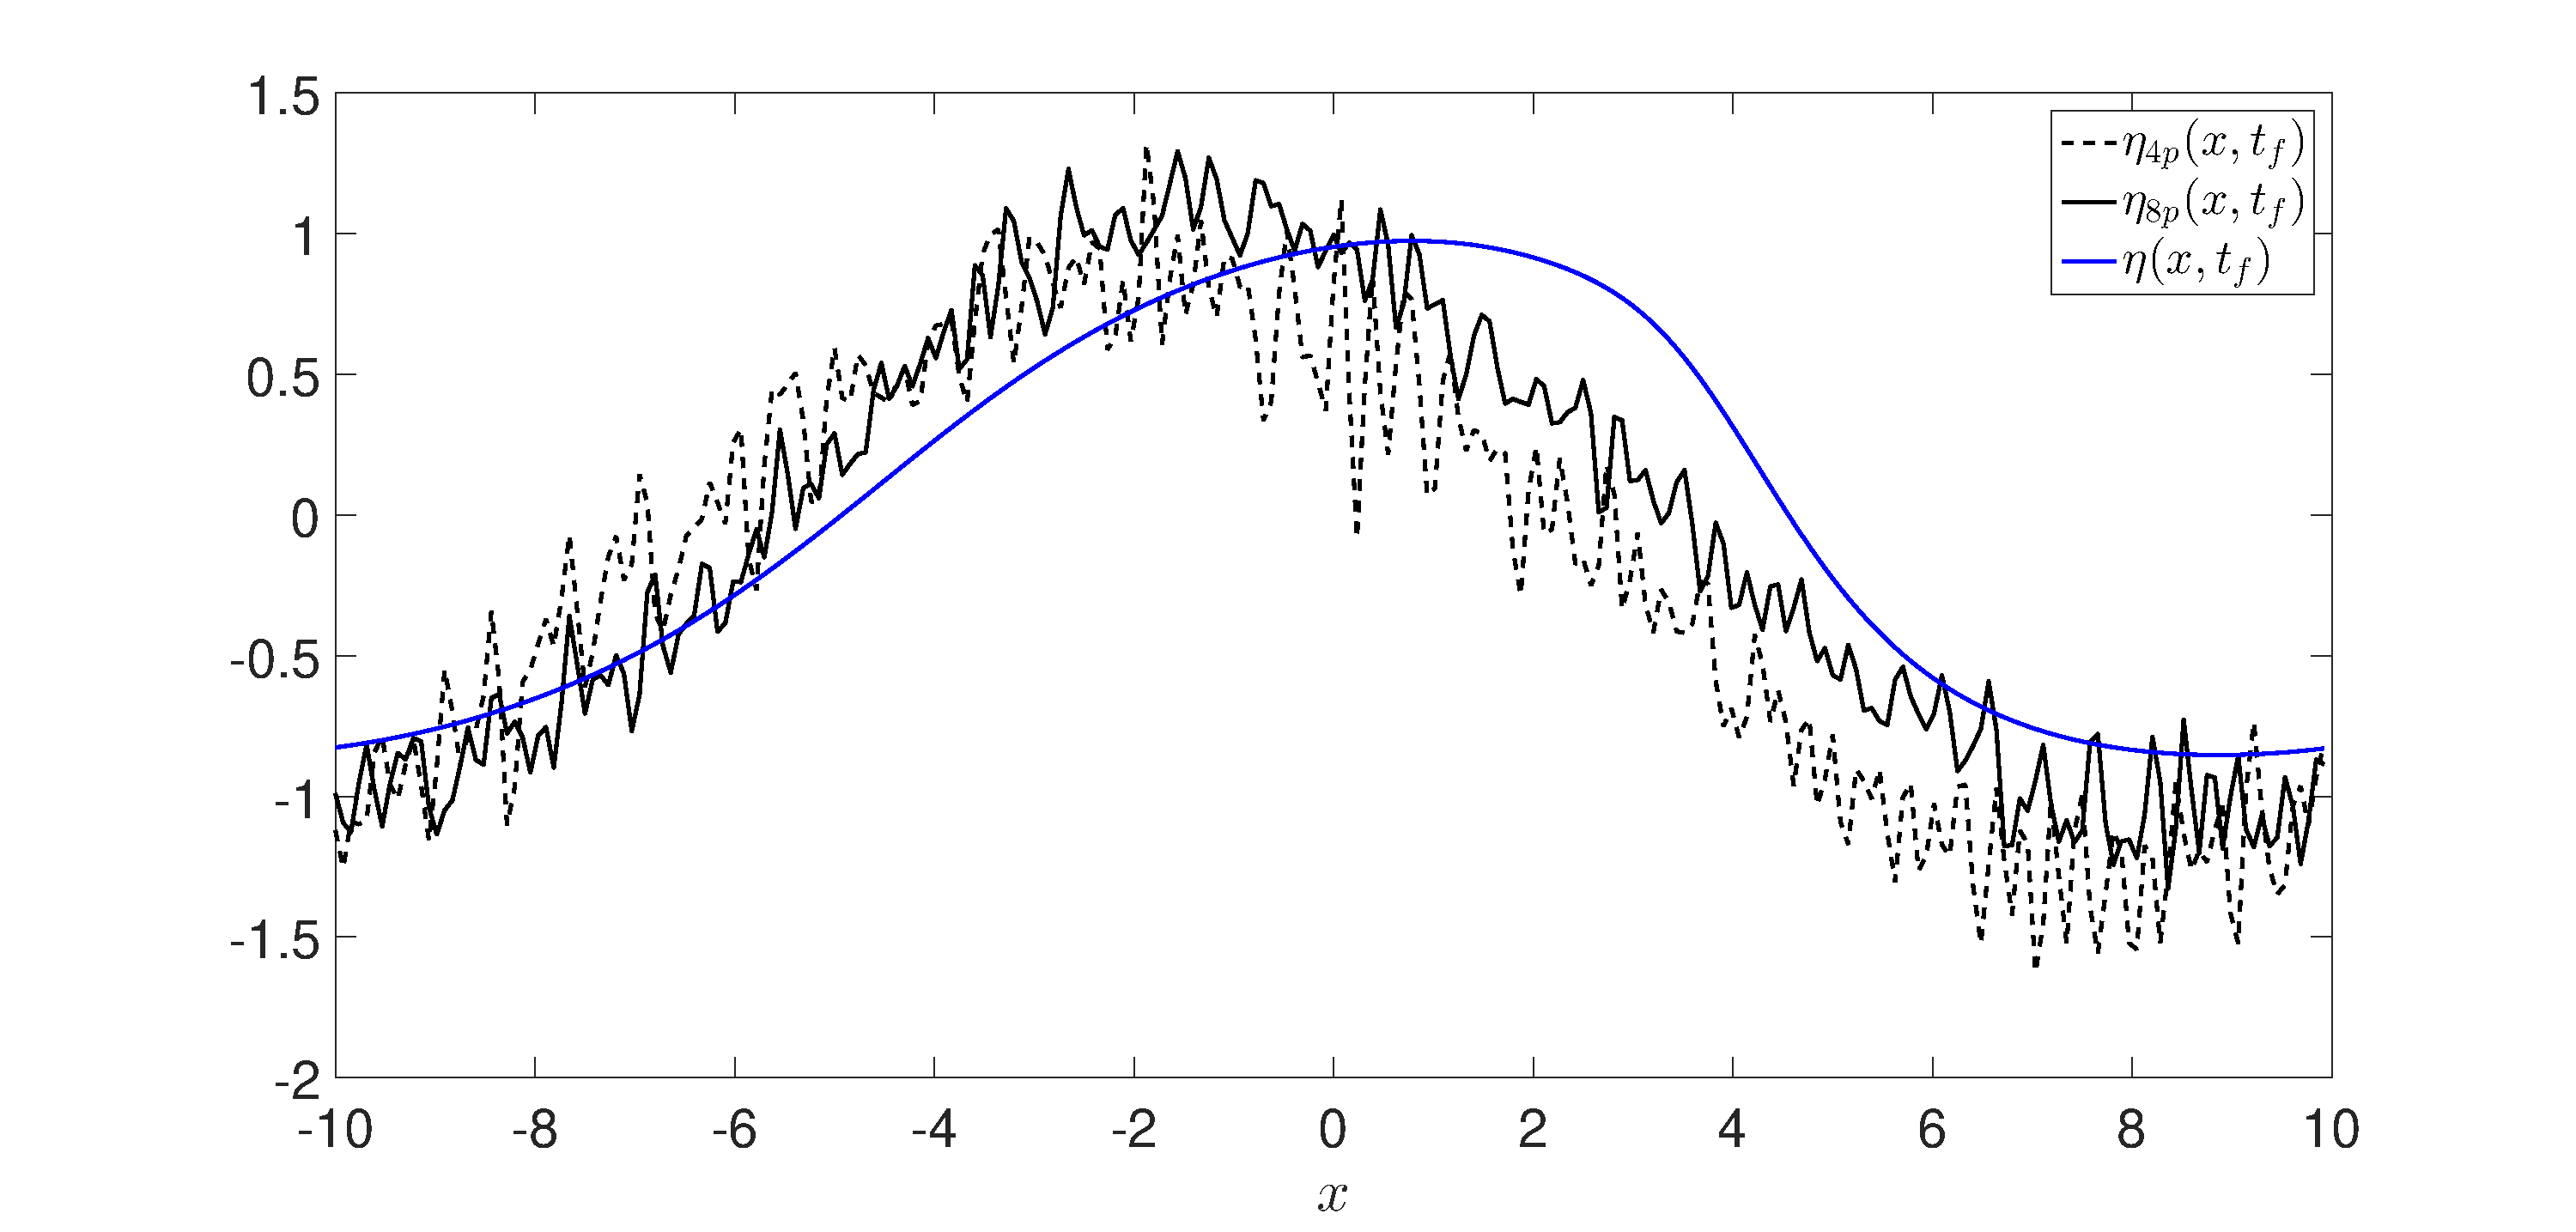
\includegraphics[width=.95\textwidth]{Images/wave_tf_20_sig_pt1_4_vs8pplates_Mval_1} \\
(a)\\
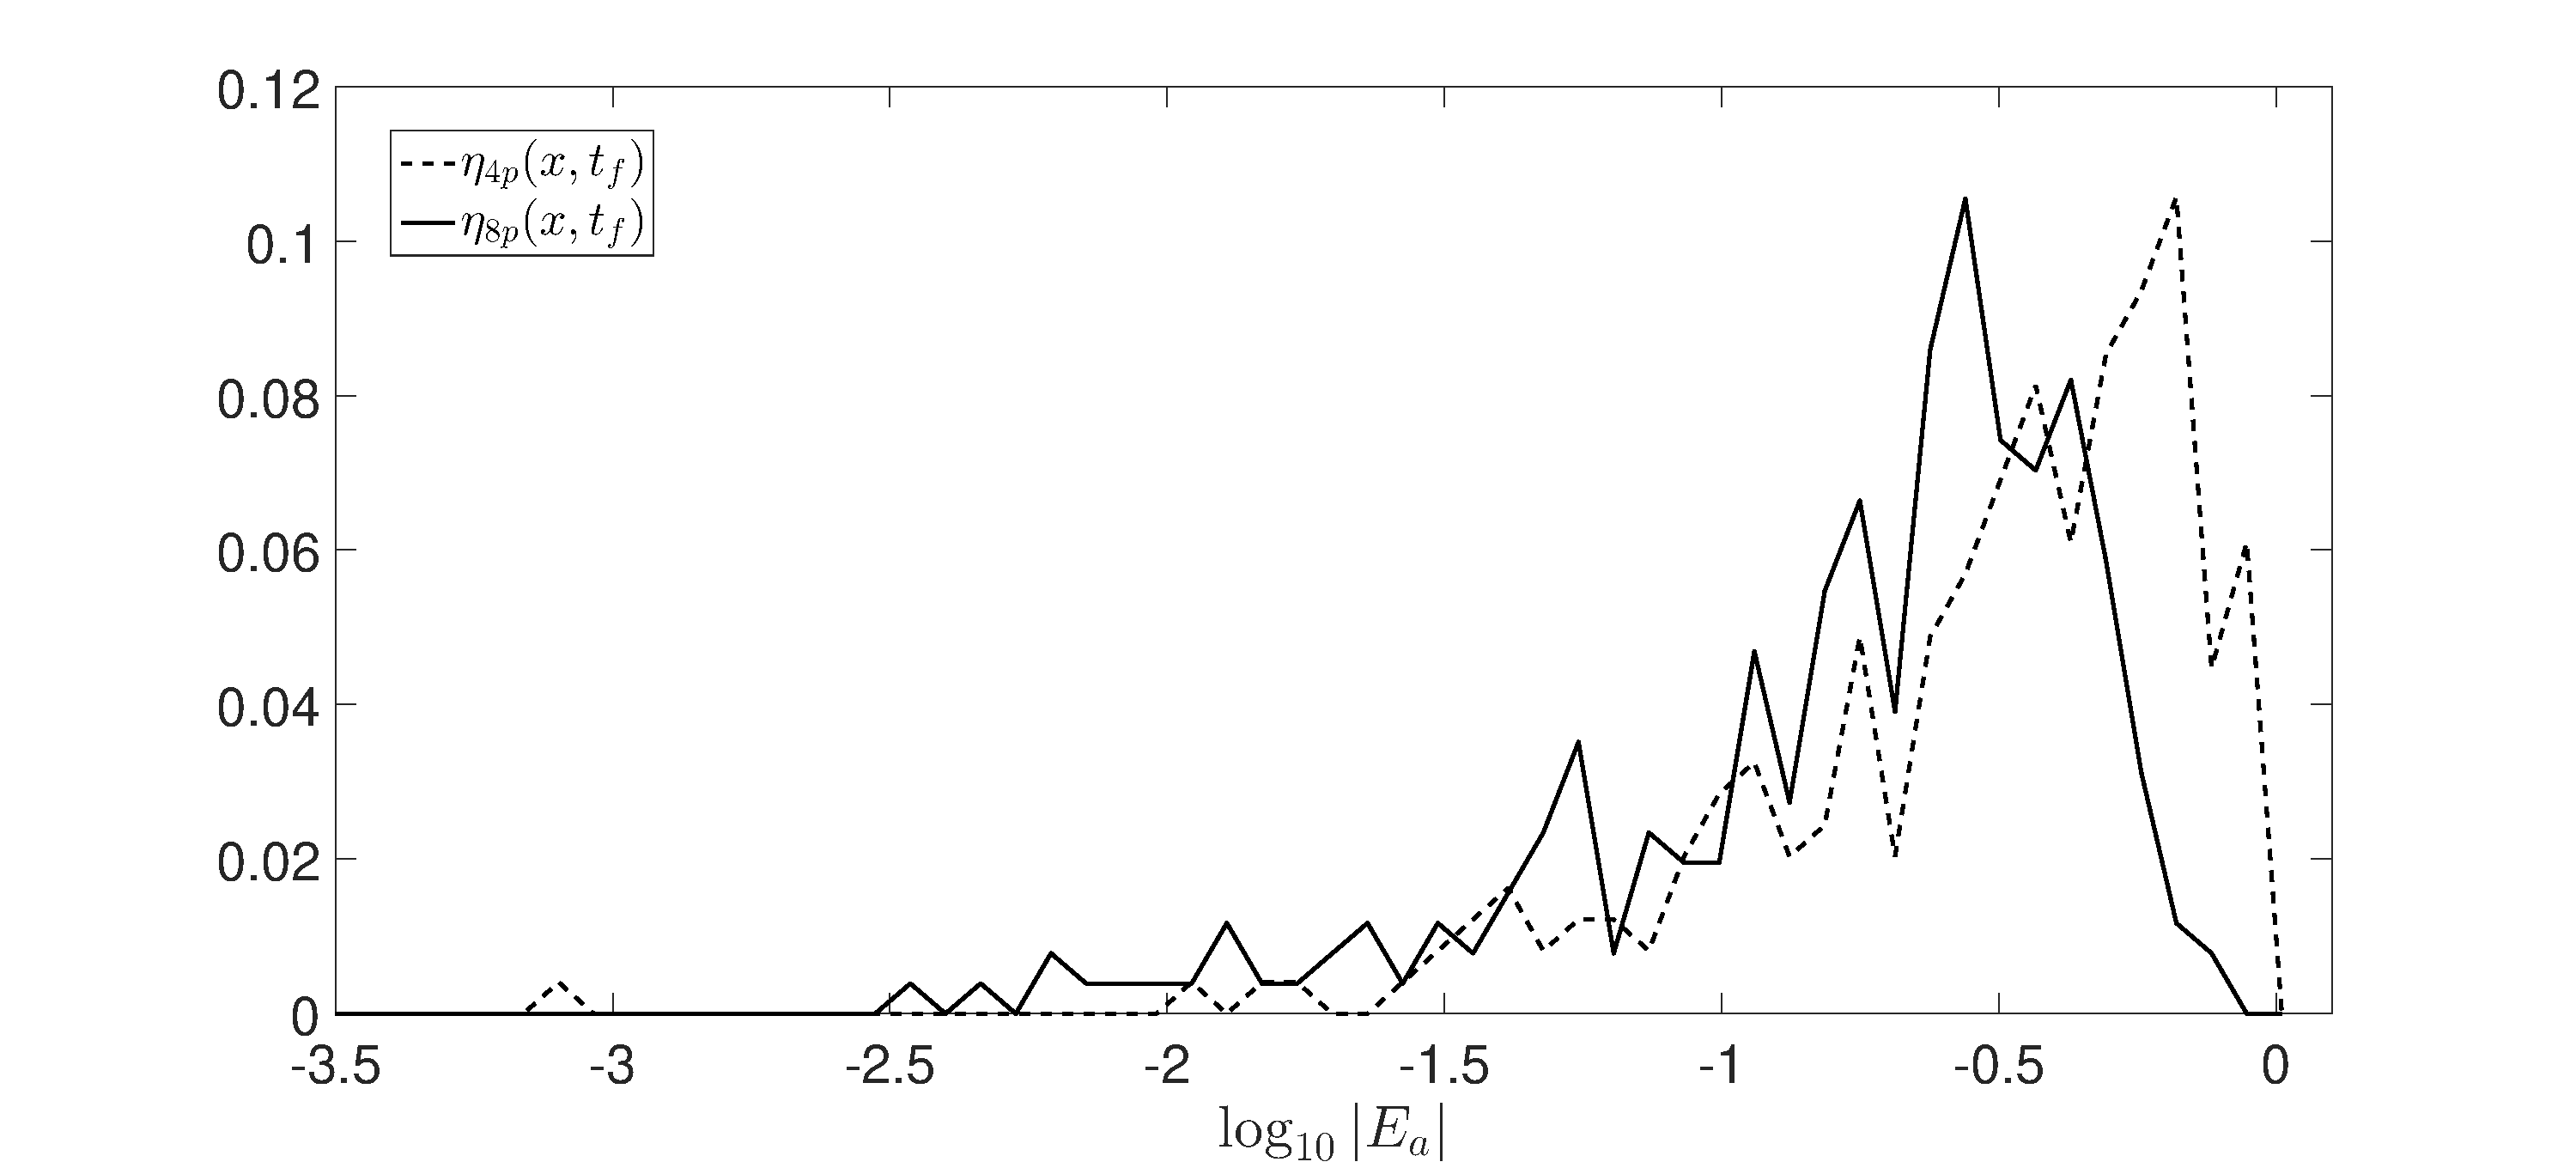
\includegraphics[width=.95\textwidth]{Images/histogram_tf_20_sig_pt1_4_vs8pplates_Mval_1}\\
(b)\\
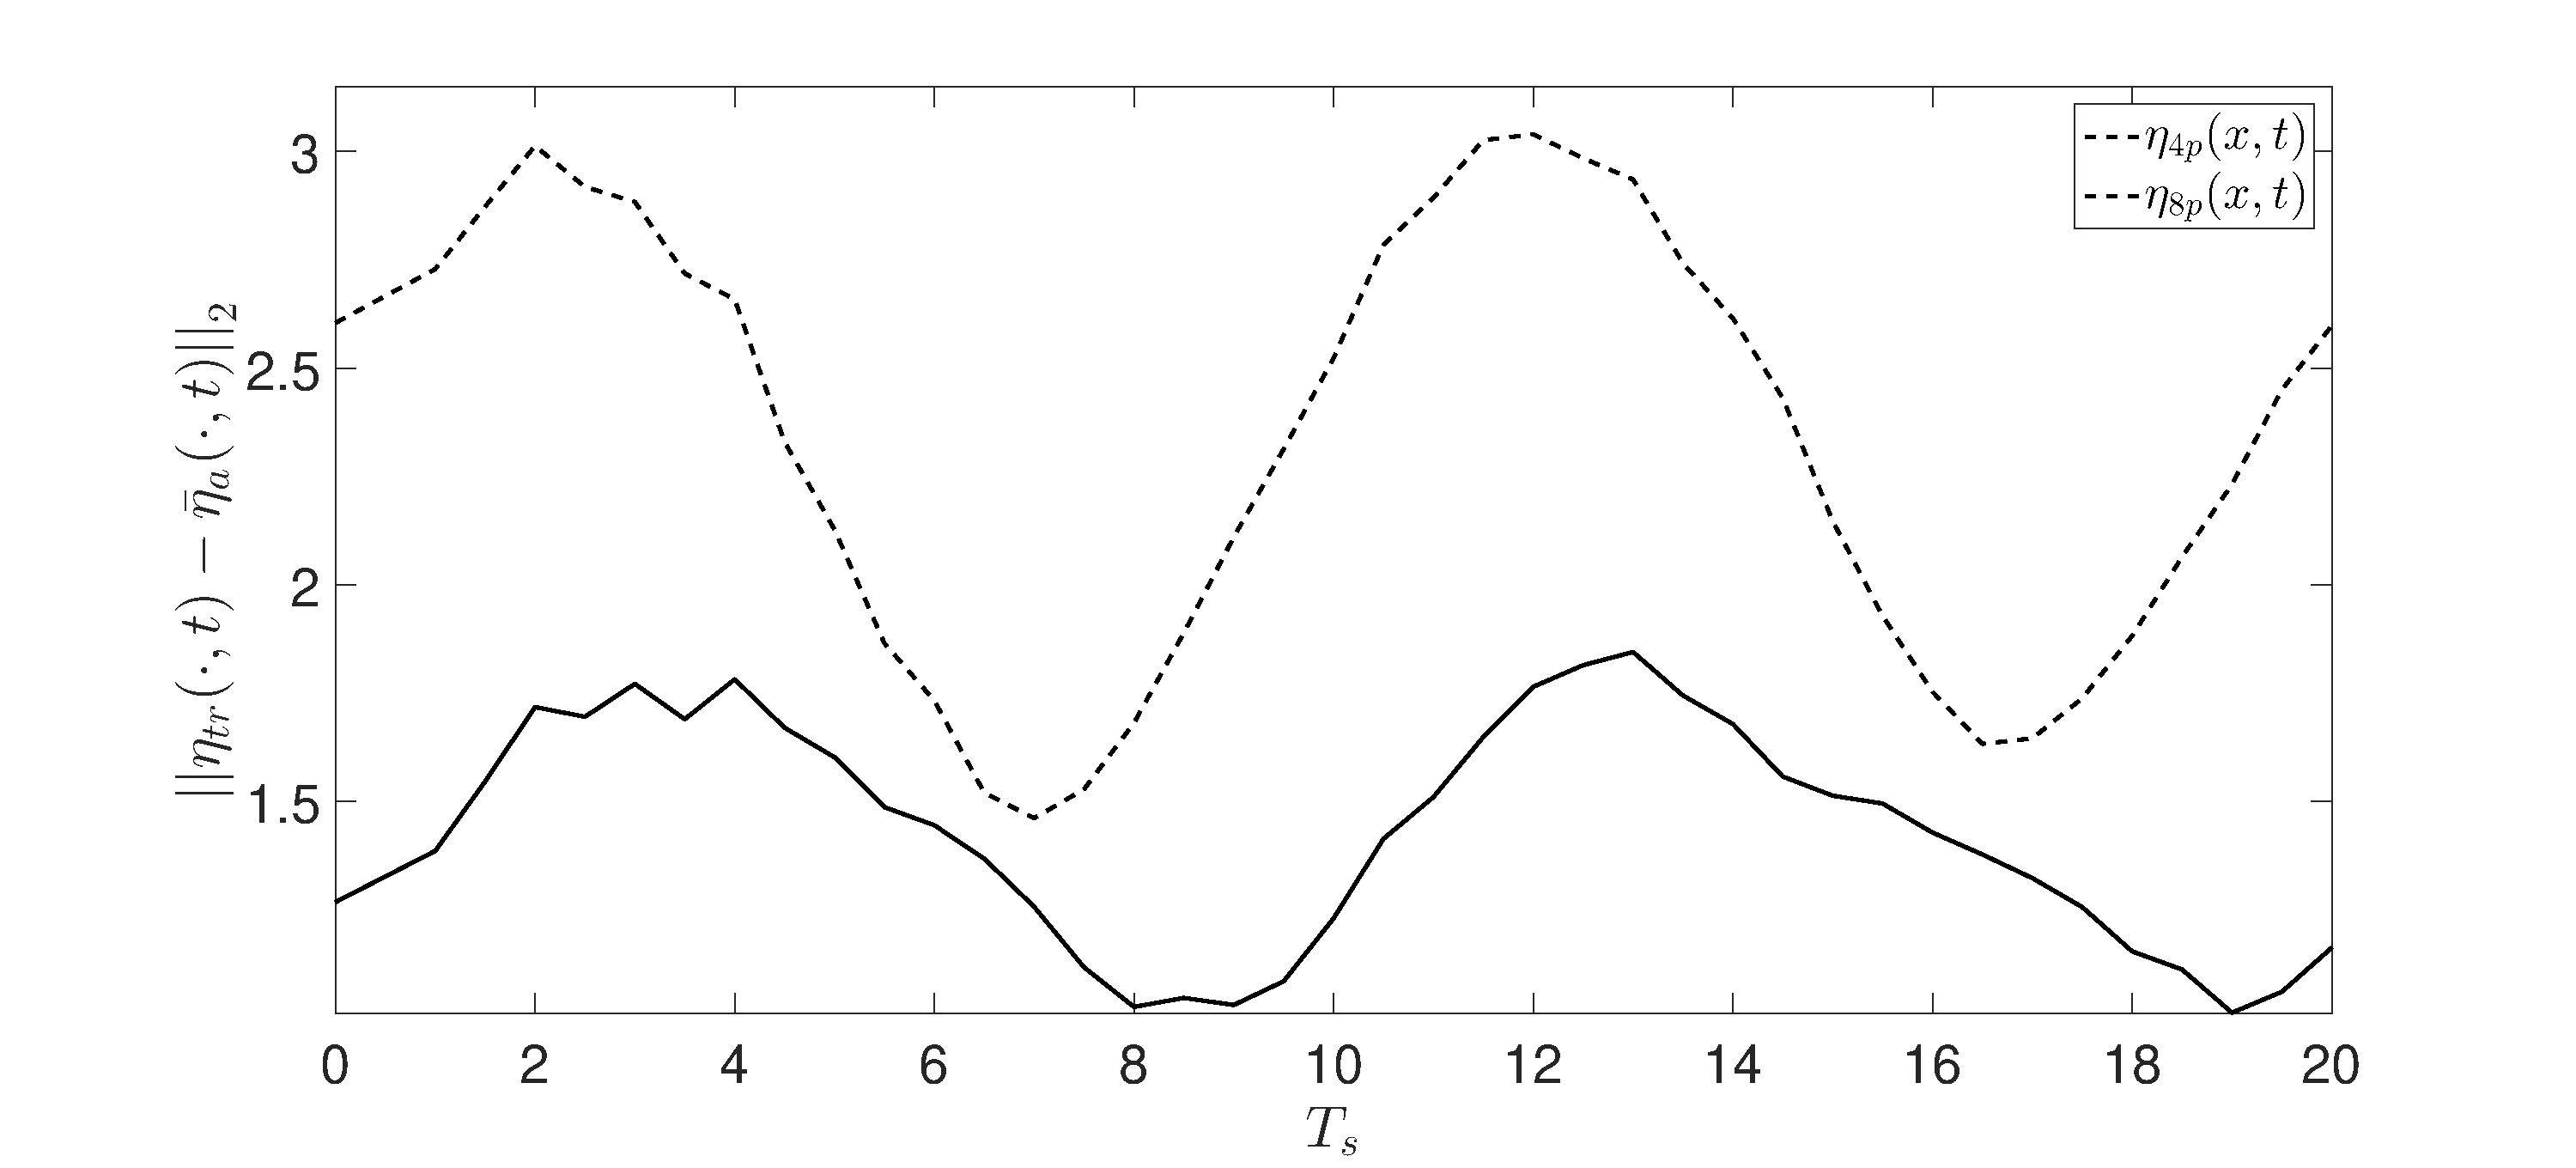
\includegraphics[width=.95\textwidth]{Images/rmserr_tf_20_sig_pt1_4_vs8pplates_Mval_1}\\
(c)
\end{tabular}
\caption{{\bf Eularian Assimilation} - For $M=1$, $dt_{s}=.5$, with four plates (--) compared to eight (-), we have the wave profiles at $t_{f}=20$ (a), a histogram of the log of the pointwise error (b), and the root-square error at every sampling time (c).} 
\label{fig:Mval_1}
\end{figure}

We then look at the impact of including higher-order nonlinearity by setting $M=14$.  We see the results of this in Figure \ref{fig:Mval_14}.  As can be seen, while there is some tendency to reduce error; see Figures \ref{fig:Mval_14} (b) and (c), including this number of terms does not materially improve the filtration process in any significant way.  This is an intriguing result hinting that while higher order effects may be critical for detailed, pointwise understandings of a process, they may essentially be so overwhelmed by noise as to be essentially useless in data assimilation algorithms.  Of course, another possibility is that the ensemble Kalman filter is so poorly adapted to the degree of nonlinearity present that it is incapable of providing significant improvements via the incorporation of data.  Finally, we may also just be paying a fundamental price for not providing any data about the velocity field at the surface.  
\begin{figure}
\centering
\begin{tabular}{c}
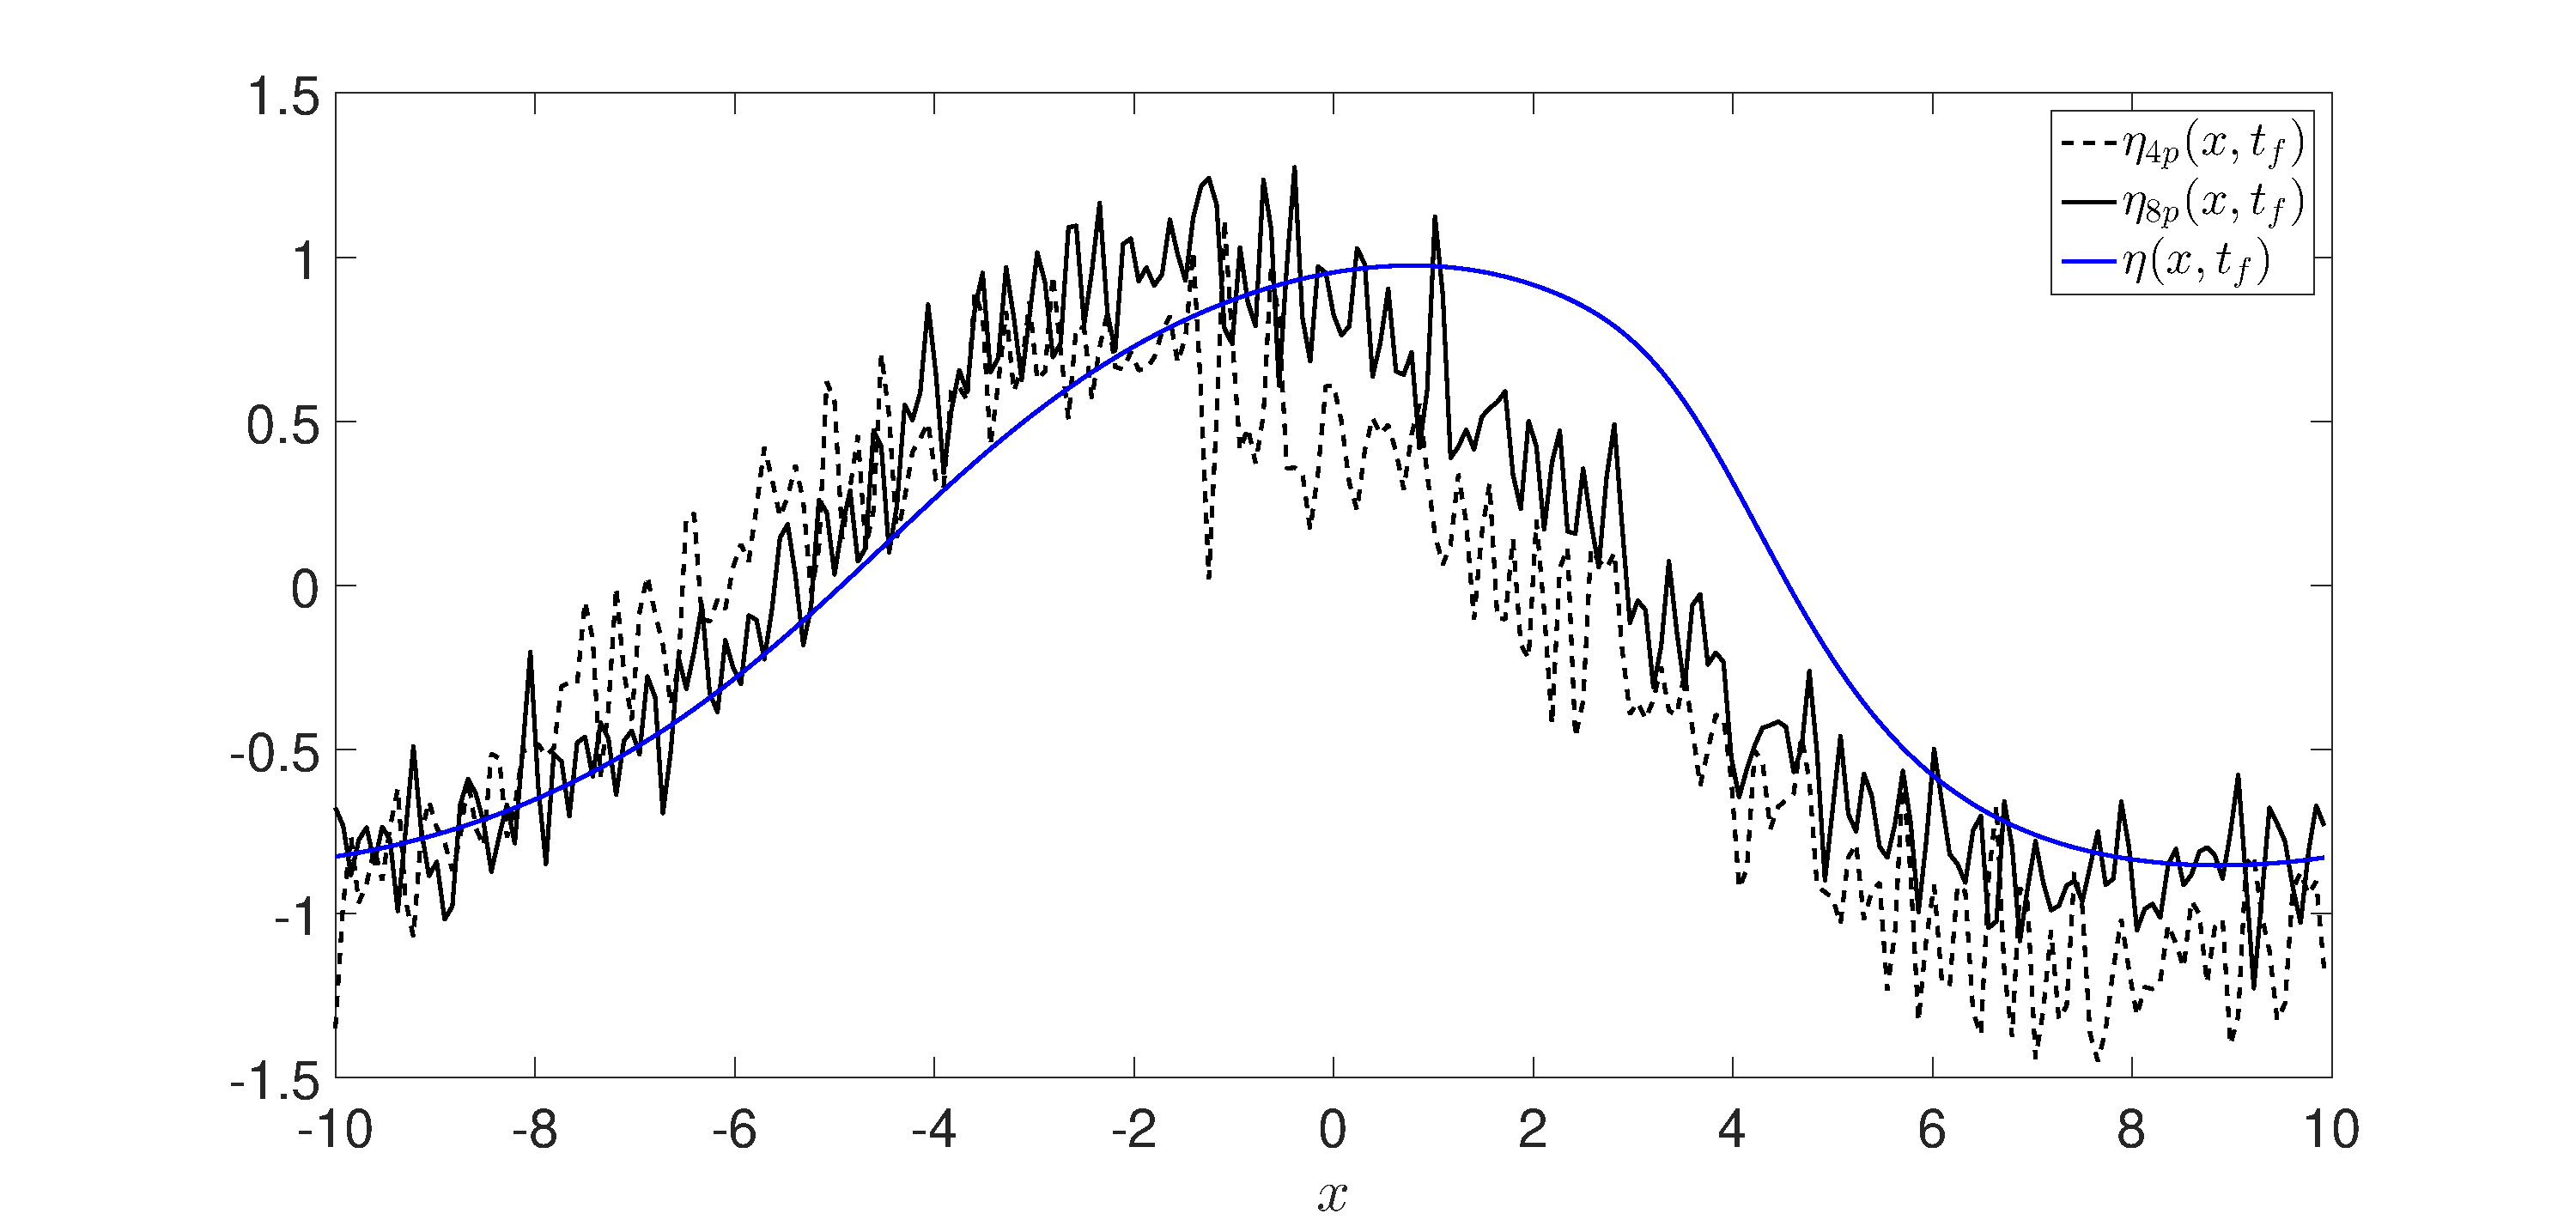
\includegraphics[width=.95\textwidth]{Images/wave_tf_20_sig_pt1_4_vs8pplates_Mval_14} \\
(a)\\
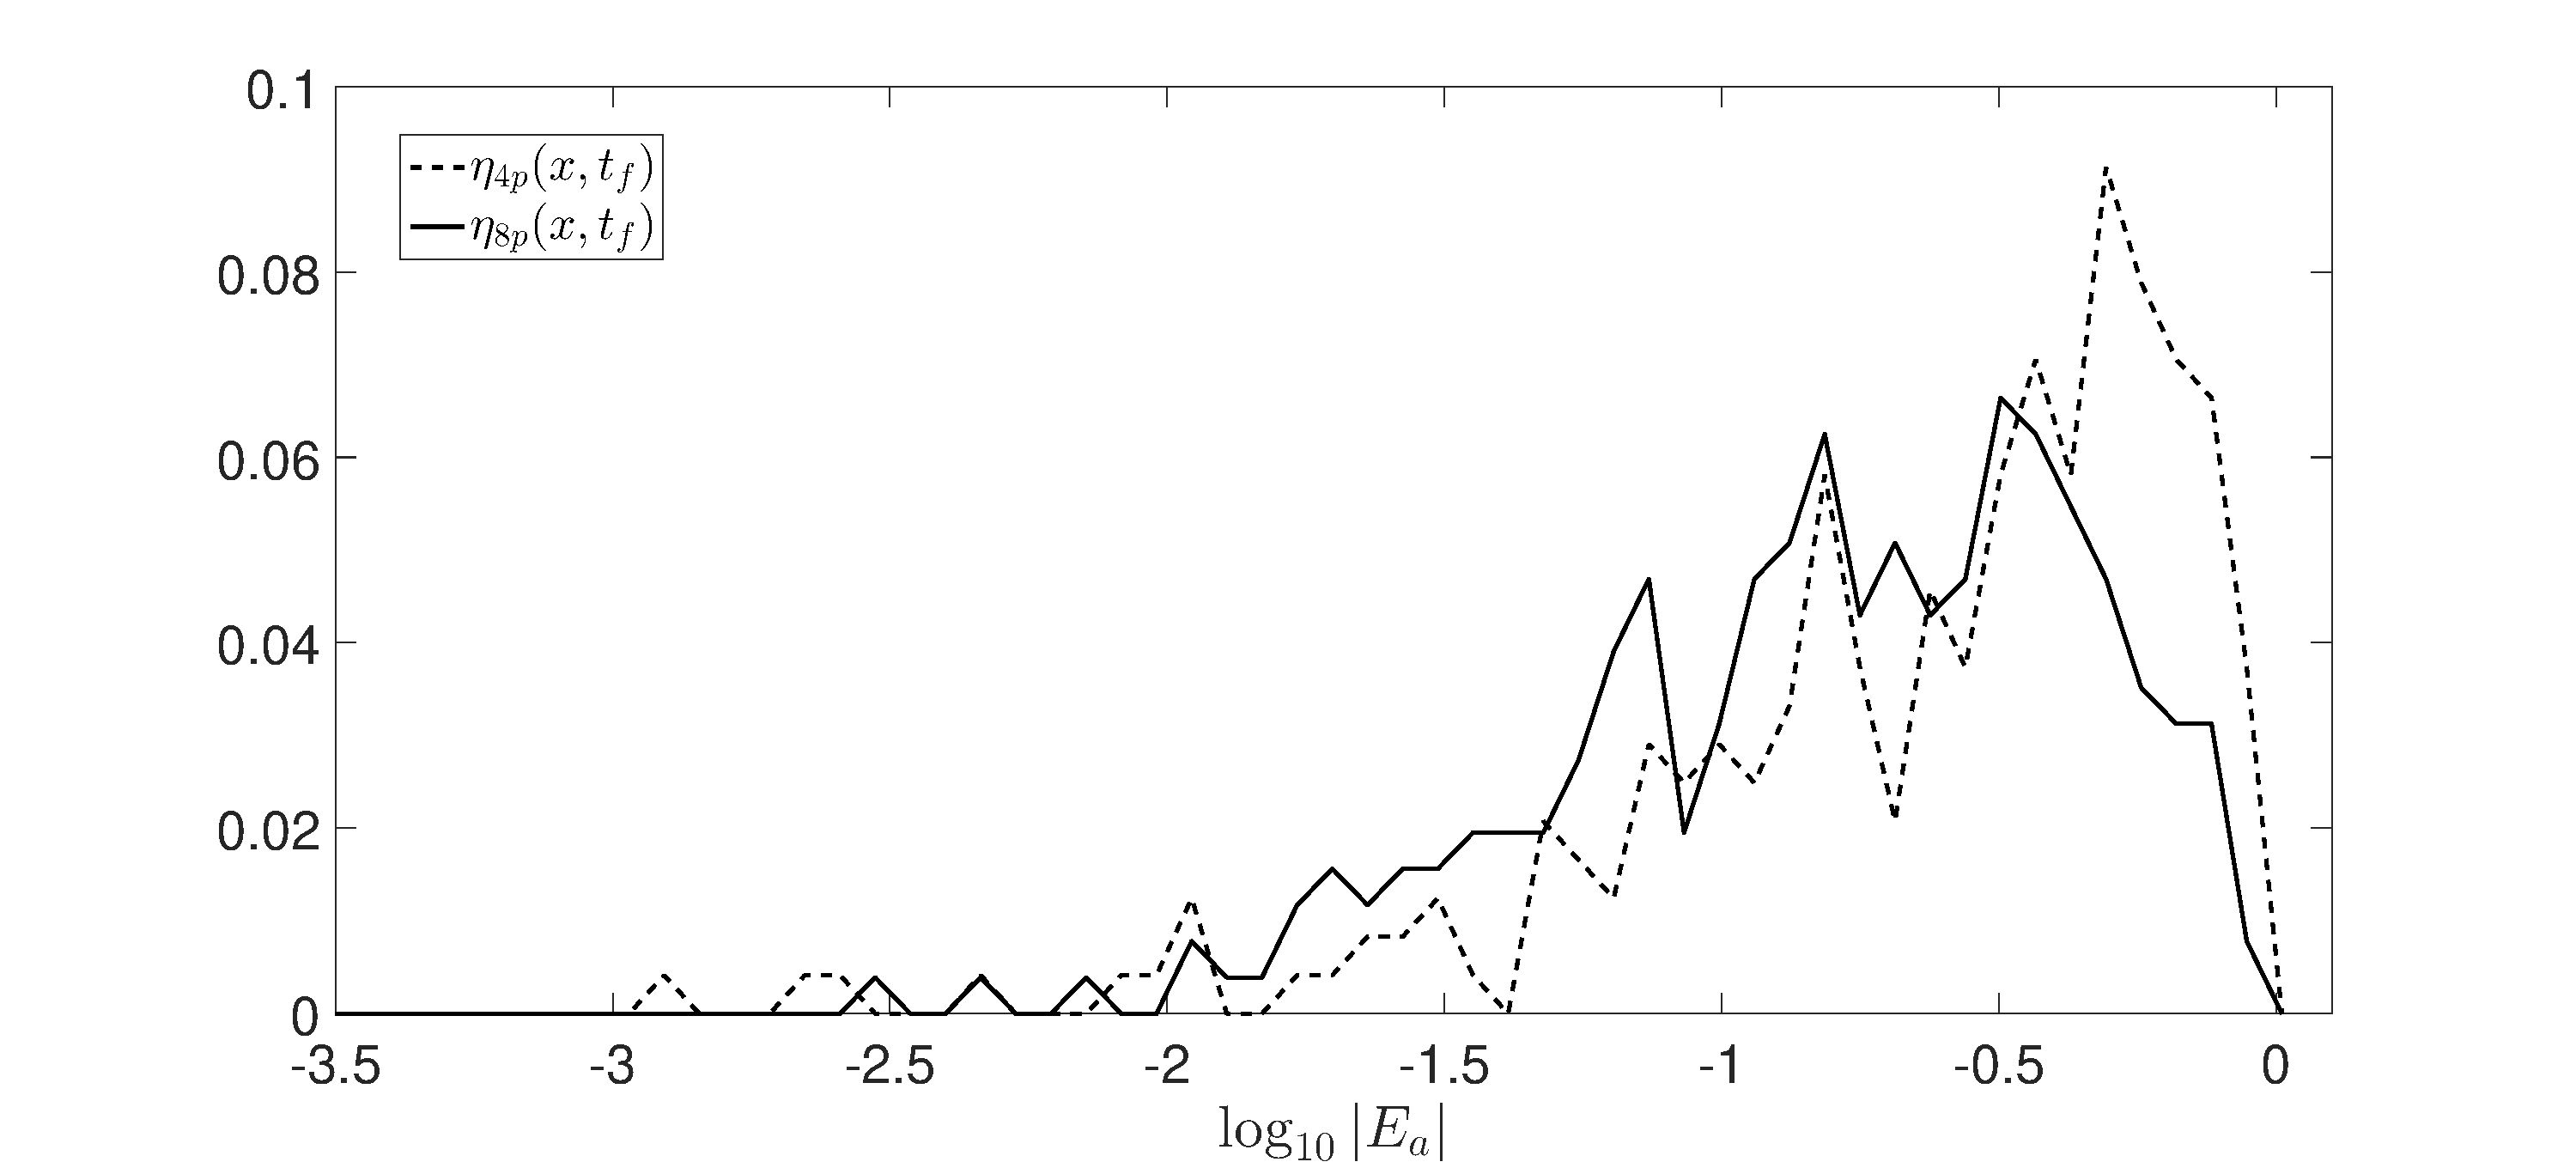
\includegraphics[width=.95\textwidth]{Images/histogram_tf_20_sig_pt1_4_vs8pplates_Mval_14}\\
(b)\\
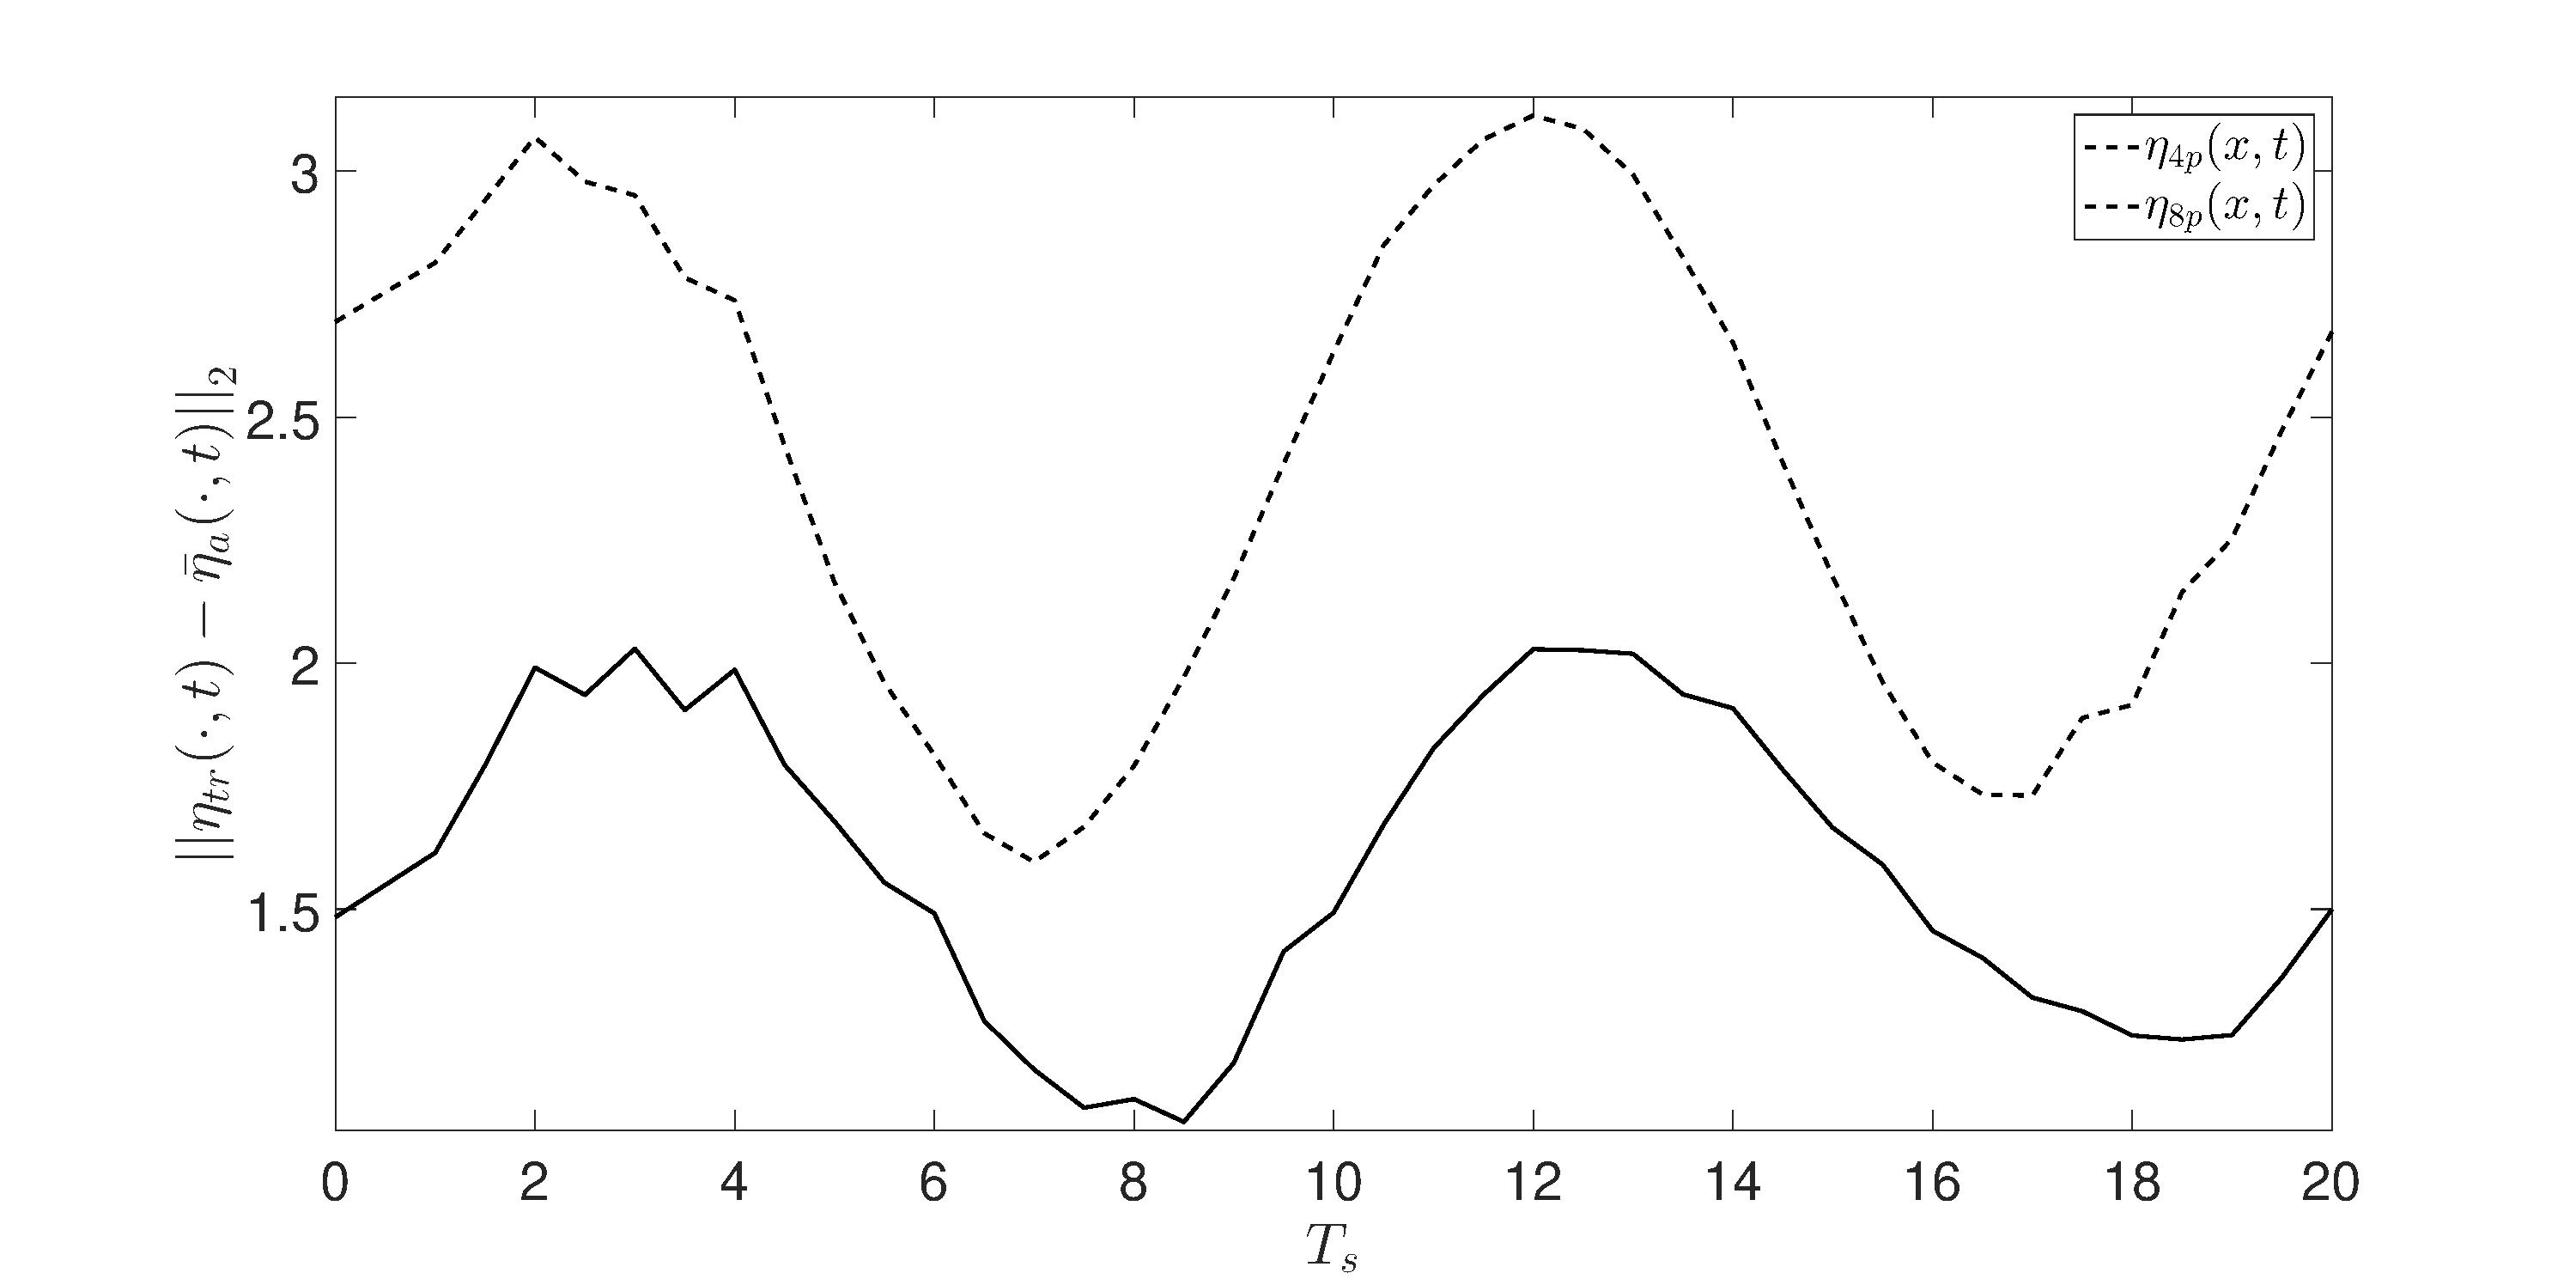
\includegraphics[width=.95\textwidth]{Images/rmserr_tf_20_sig_pt1_4_vs8pplates_Mval_14}\\
(c)
\end{tabular}
\caption{{\bf Eularian Assimilation} - For $M=14$, $dt_{s}=.5$, with four plates (--) compared to eight (-), we have the wave profiles at $t_{f}=20$ (a), a histogram of the log of the pointwise error (b), and the root-square error at every sampling time (c).} 
\label{fig:Mval_14}
\end{figure}

%%%%%%%%%%%%%%%%%%%%%%%%%%%%%%%%%%%%%%%%%%%%%%%%%%%%%%%%%%%%%%%%%%%%%%%%%%%%%%%%%%%


\subsection*{Lagrangian Data Assimilation Results}

An obvious question is whether using Lagrangian information coming from freely moving floats on the surface provide a more accurate means of filtering.  As seen in Figures \ref{fig:Mval_1_lagran} and \ref{fig:Mval_14_lagran} this does not appear to be the case.  The distribution of errors and the 2-norm of the error at sampling times is essentially the same as in the Eularian case.  Arguably, by comparing the distributions in Figures \ref{fig:Mval_1} (b) and \ref{fig:Mval_14} (b) to those in Figures \ref{fig:Mval_1_lagran} (b) and \ref{fig:Mval_14_lagran} (b), the Eularian assimilation scheme pushes the peak of the error down relative to the Lagrangian scheme.  Again though, nonlinearity seems to be beyond the reach of the ensemble Kalman filter, and so whether this difference in behavior between Eularian and Lagrangian schemes is a general feature or specific to the Kalman filter is a question for future study.   

\begin{figure}
	\centering
	\begin{tabular}{c}
		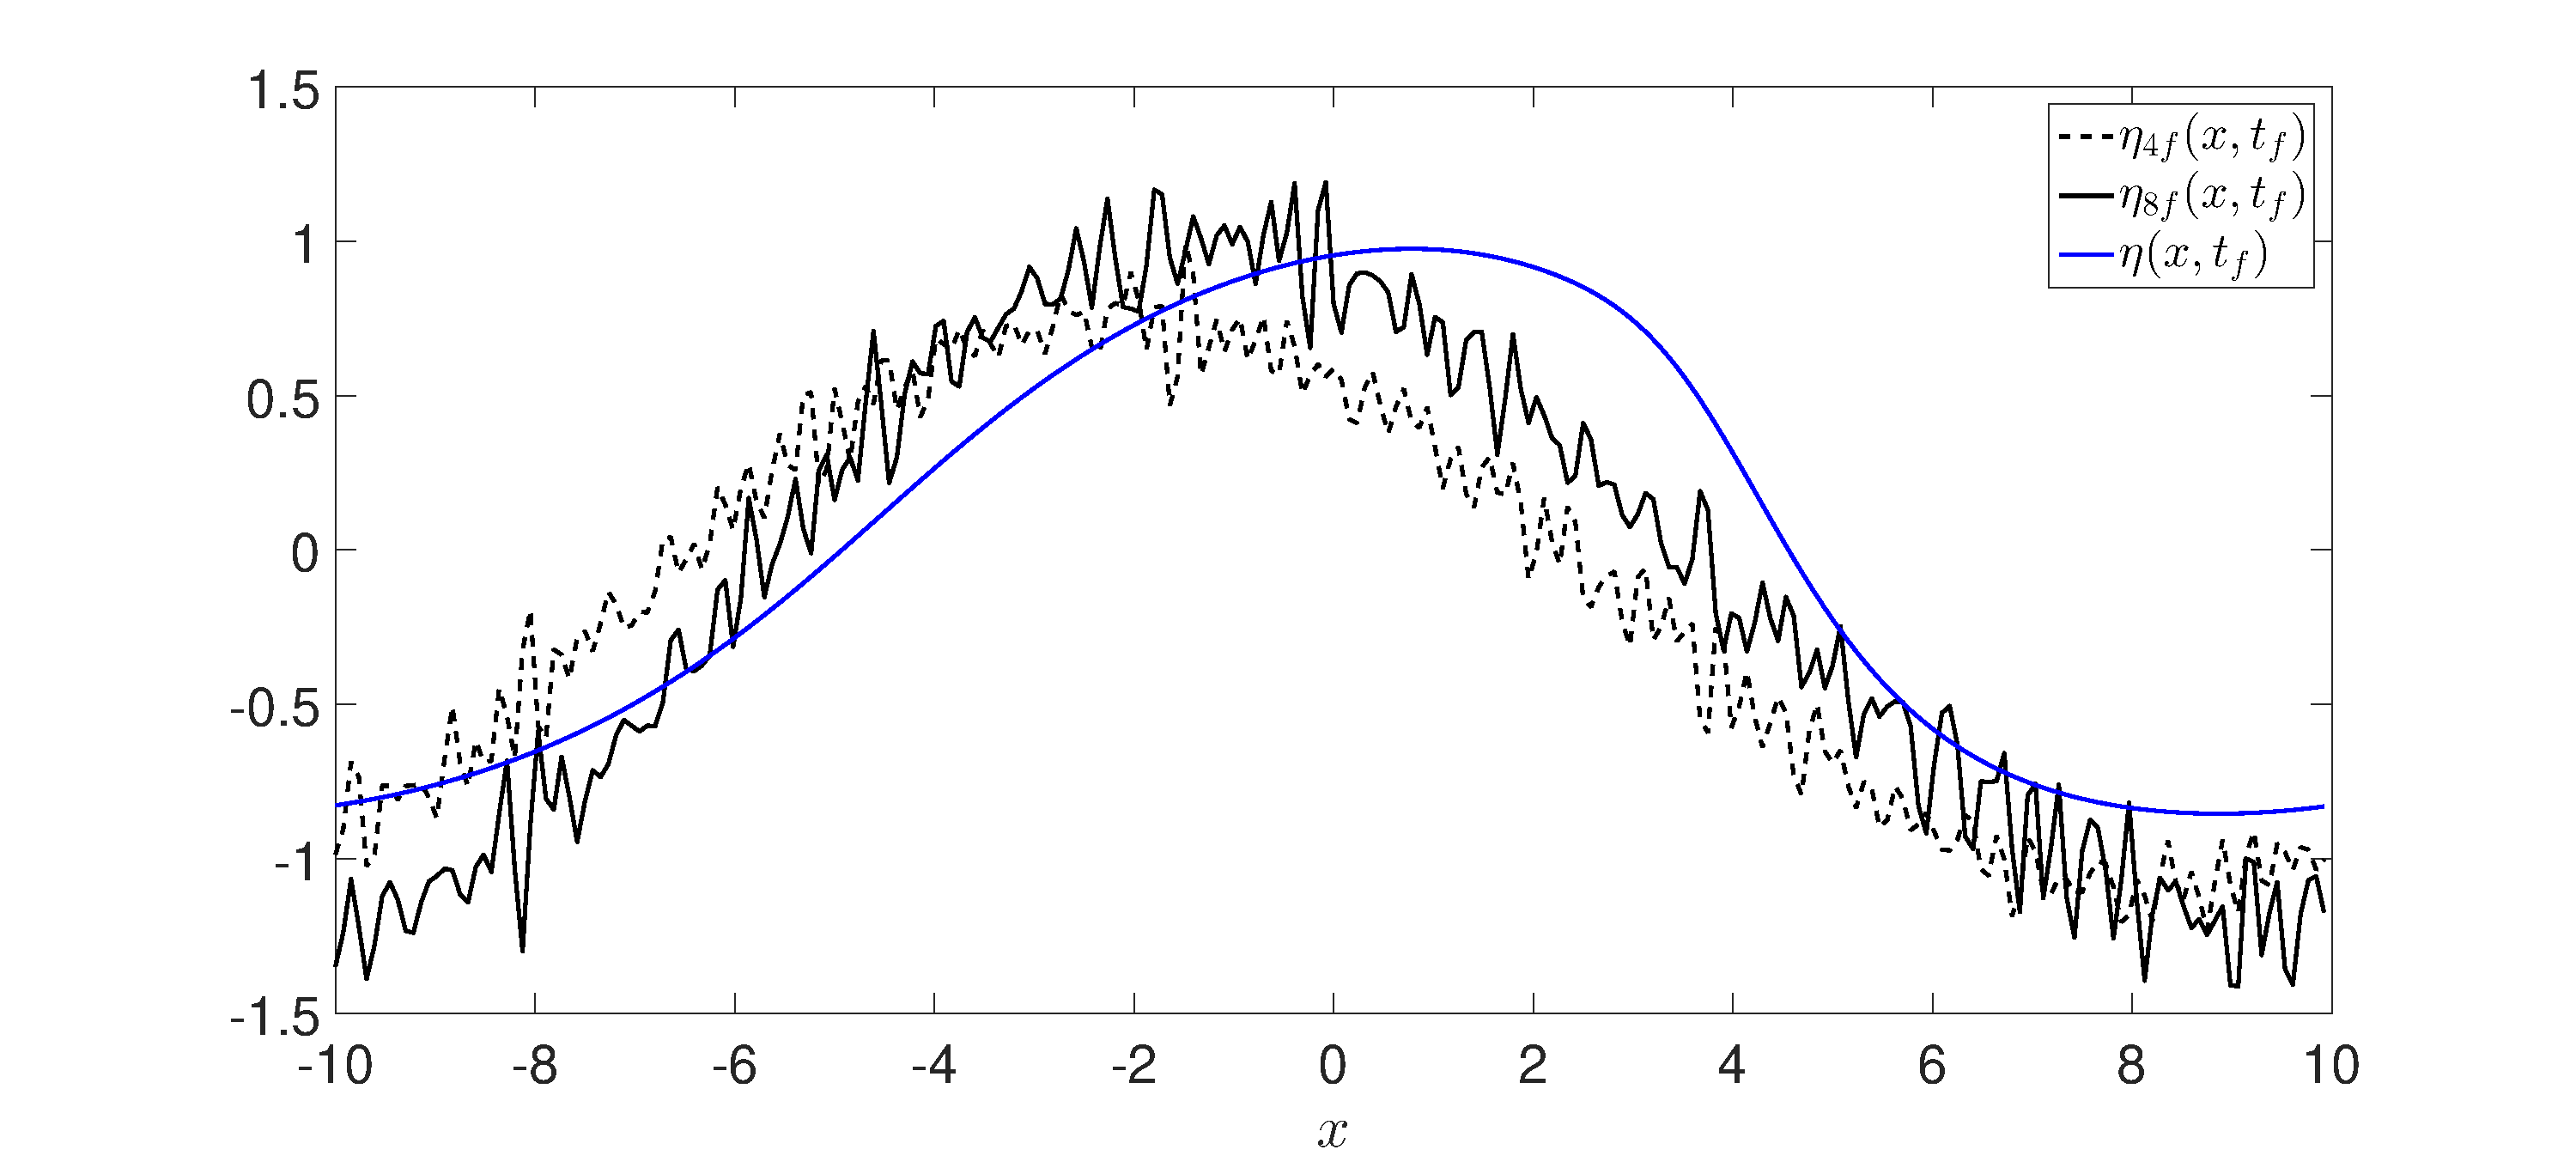
\includegraphics[width=.95\textwidth]{Images/wave_tf_20_sig_pt1_4_vs8floats_Mval_1} \\
		(a)\\
		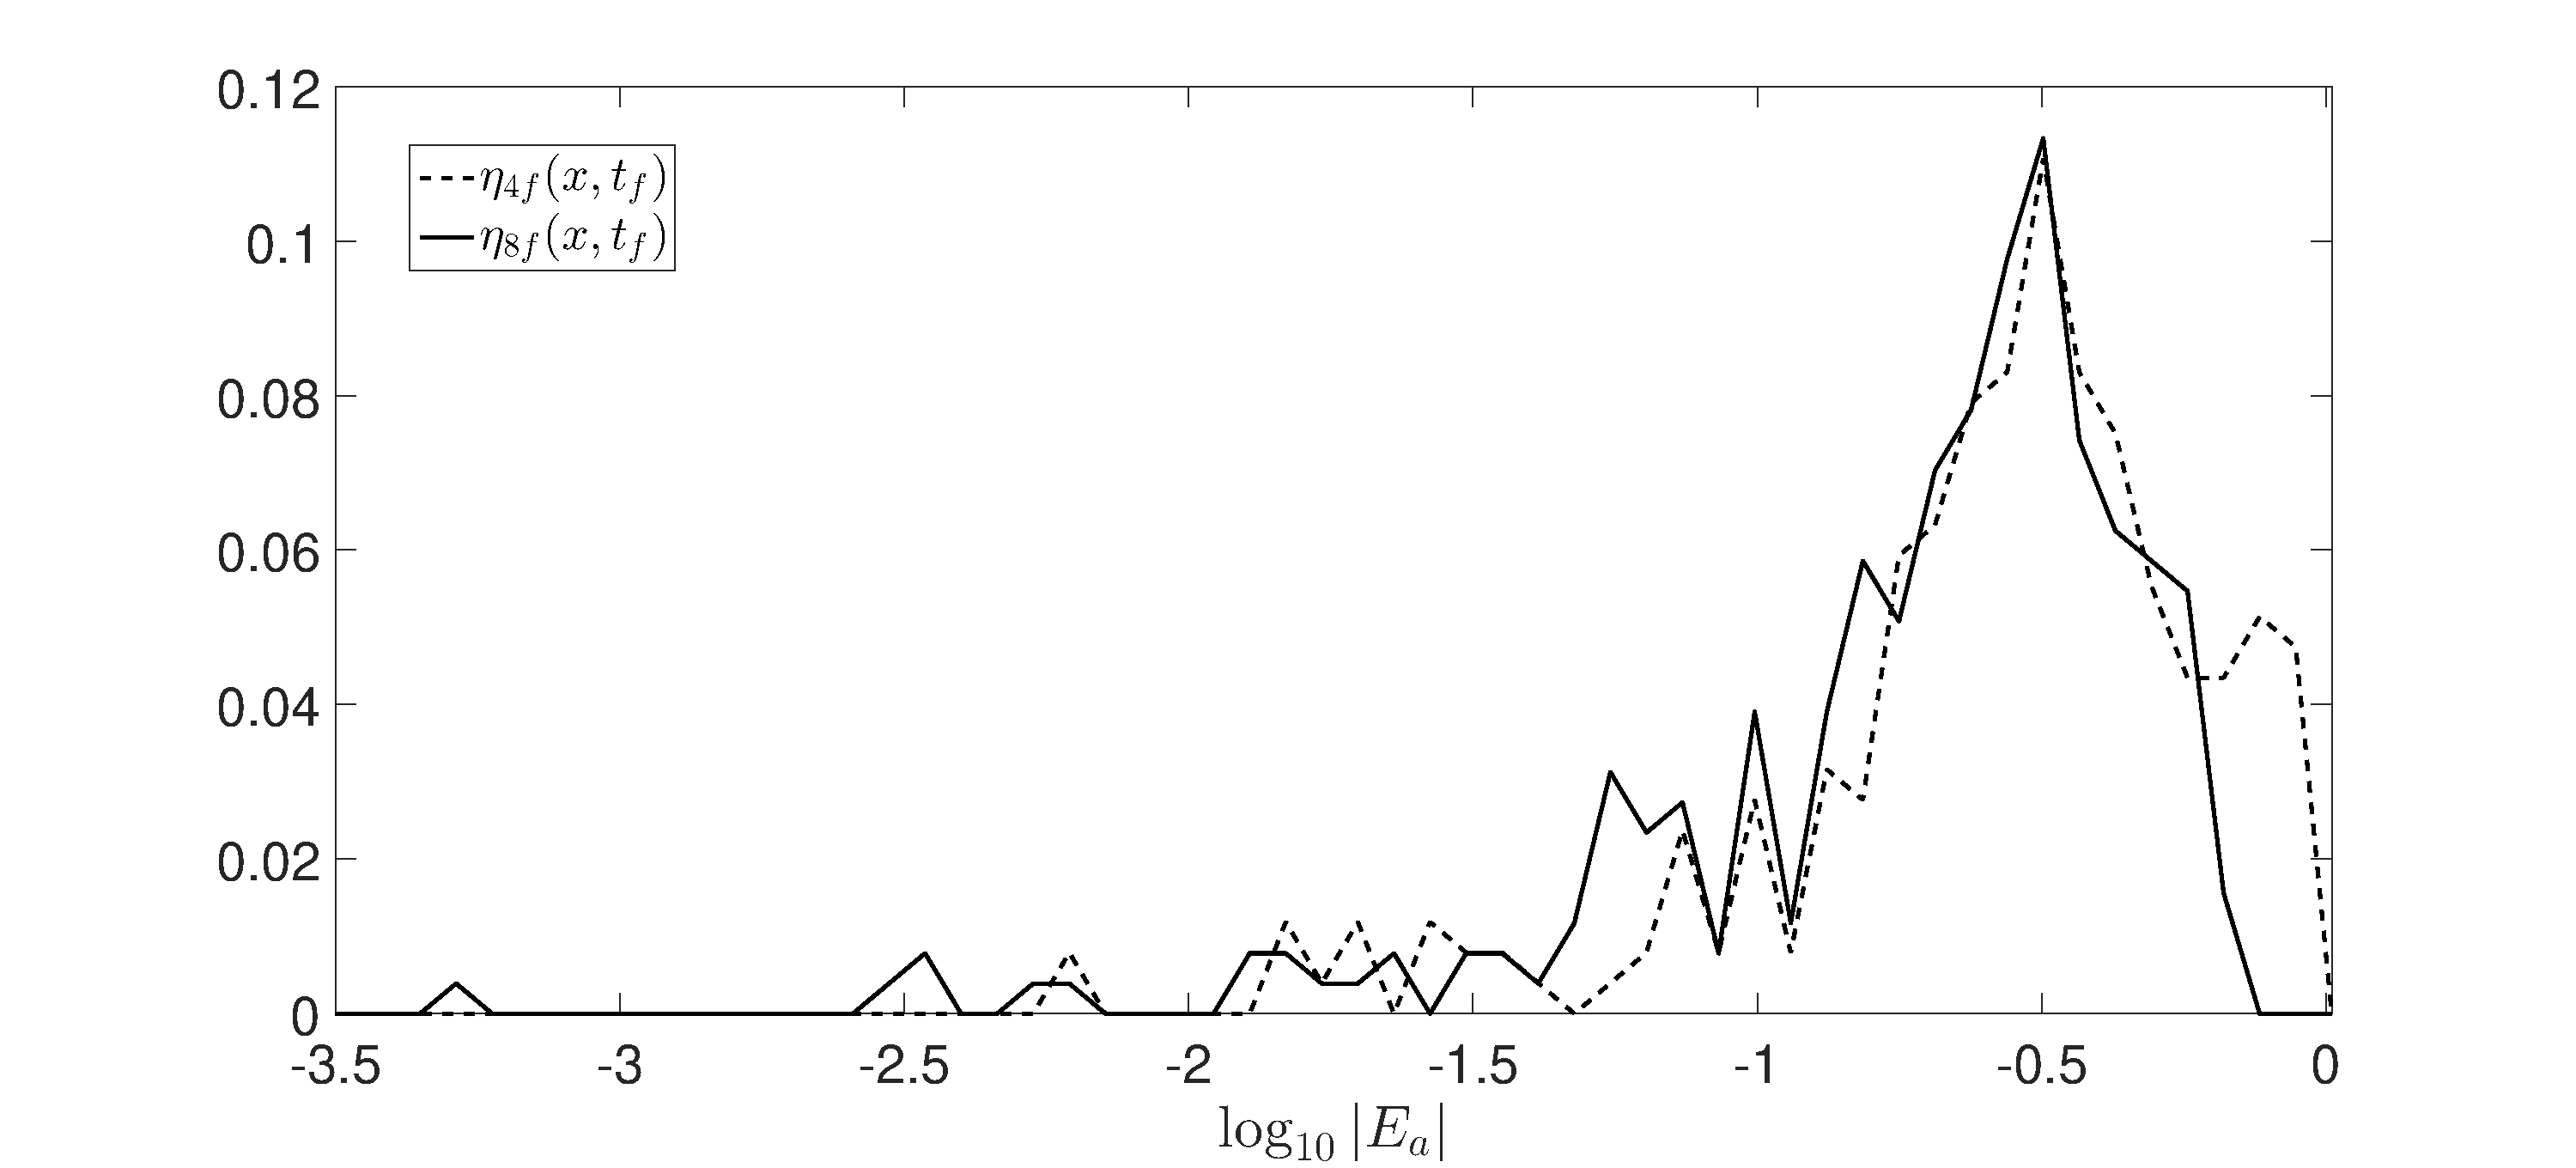
\includegraphics[width=.95\textwidth]{Images/histogram_tf_20_sig_pt1_4_vs_8floats_Mval_1}\\
		(b)\\
		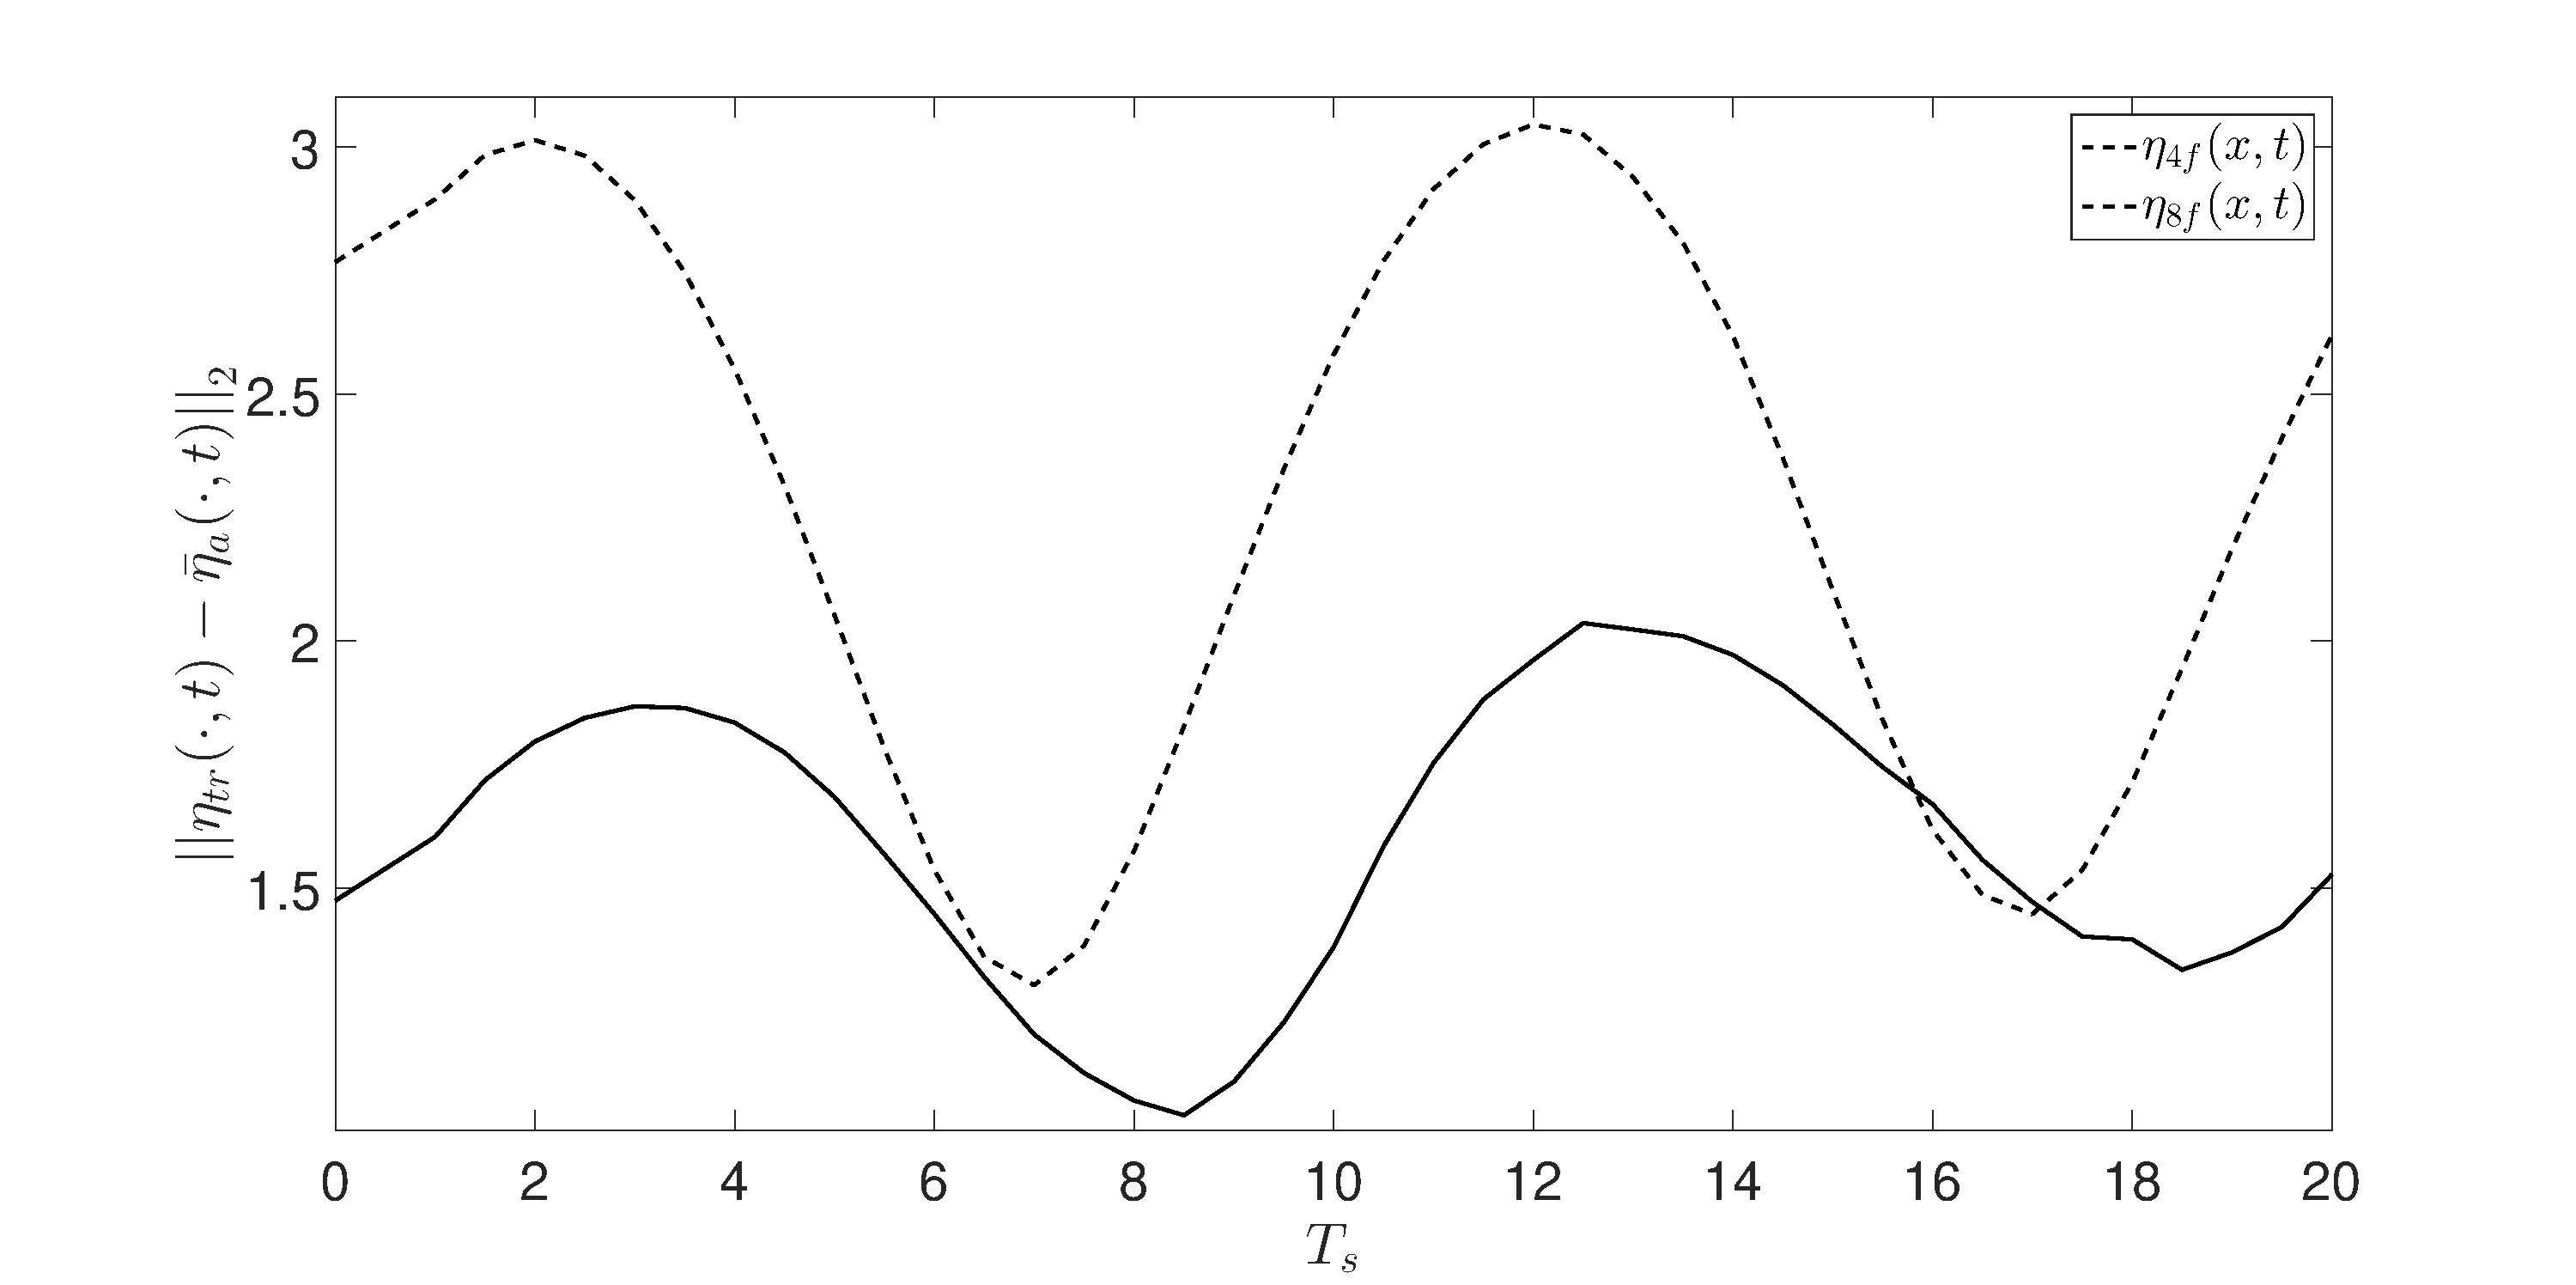
\includegraphics[width=.95\textwidth]{Images/rmserr_tf_20_sig_pt1_4_vs8floats_Mval_1}\\
		(c)
	\end{tabular}
	\caption{{\bf Lagrangian Assimilation} - For $M=1$, $dt_{s}=.5$, with four floats (--) compared to eight (-), we have the wave profiles at $t_{f}=20$ (a), a histogram of the log of the pointwise error (b), and the root-mean square error at every sampling time (c).} 
	\label{fig:Mval_1_lagran}
\end{figure}

\begin{figure}
	\centering
	\begin{tabular}{c}
		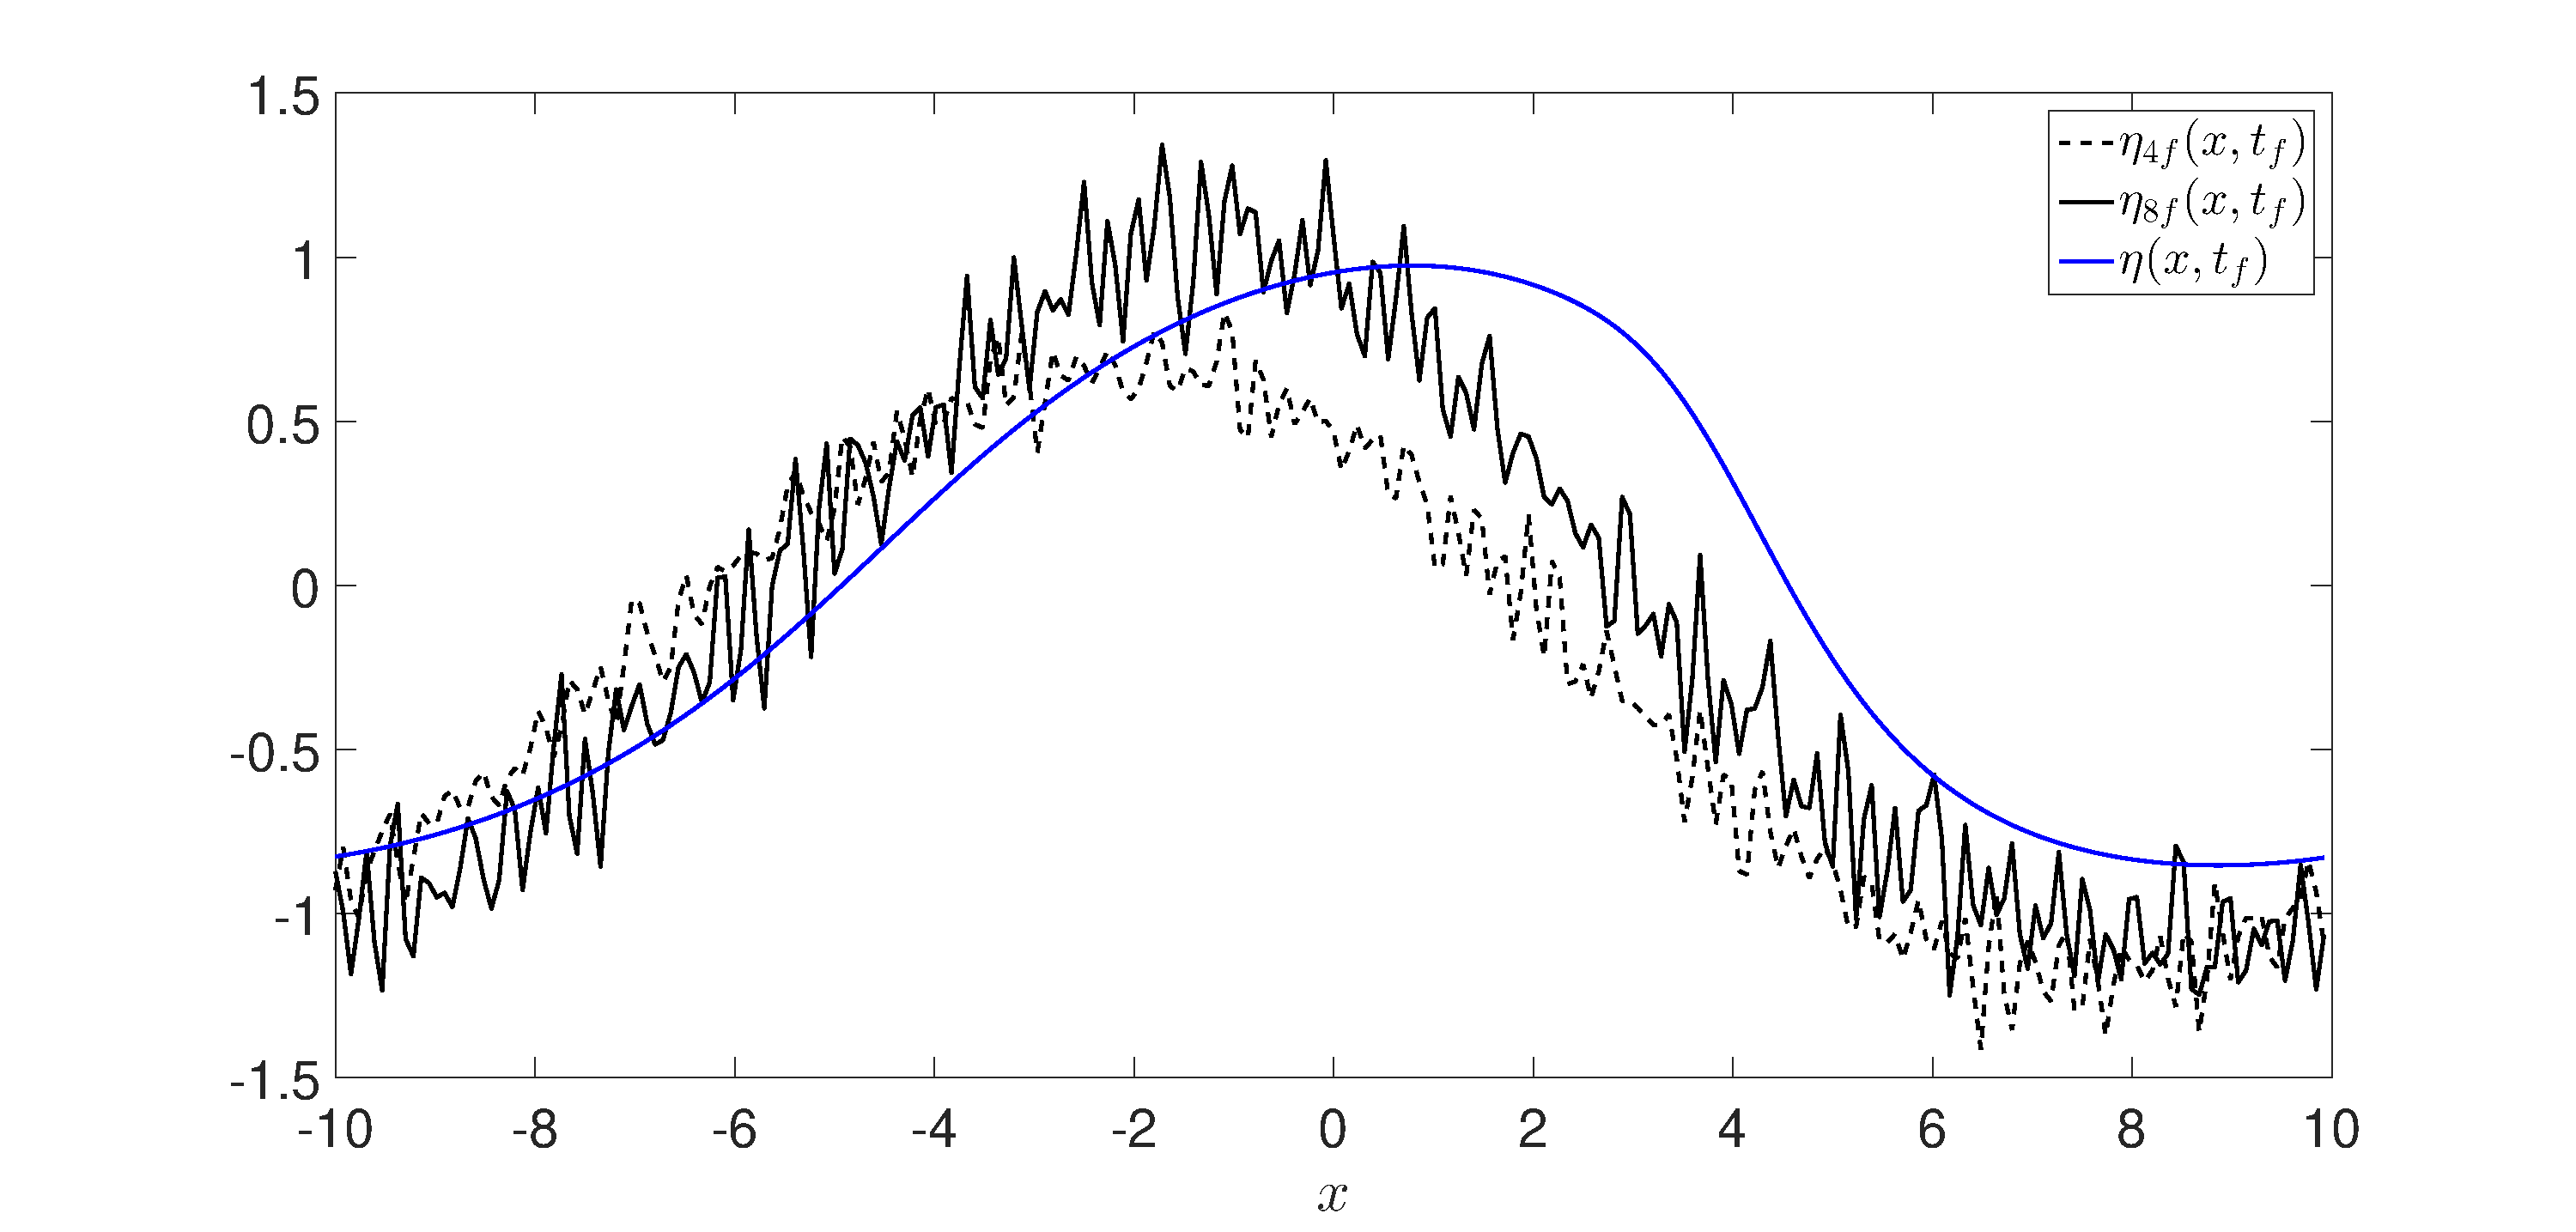
\includegraphics[width=.95\textwidth]{Images/wave_tf_20_sig_pt1_4_vs8floats_Mval_14} \\
		(a)\\
		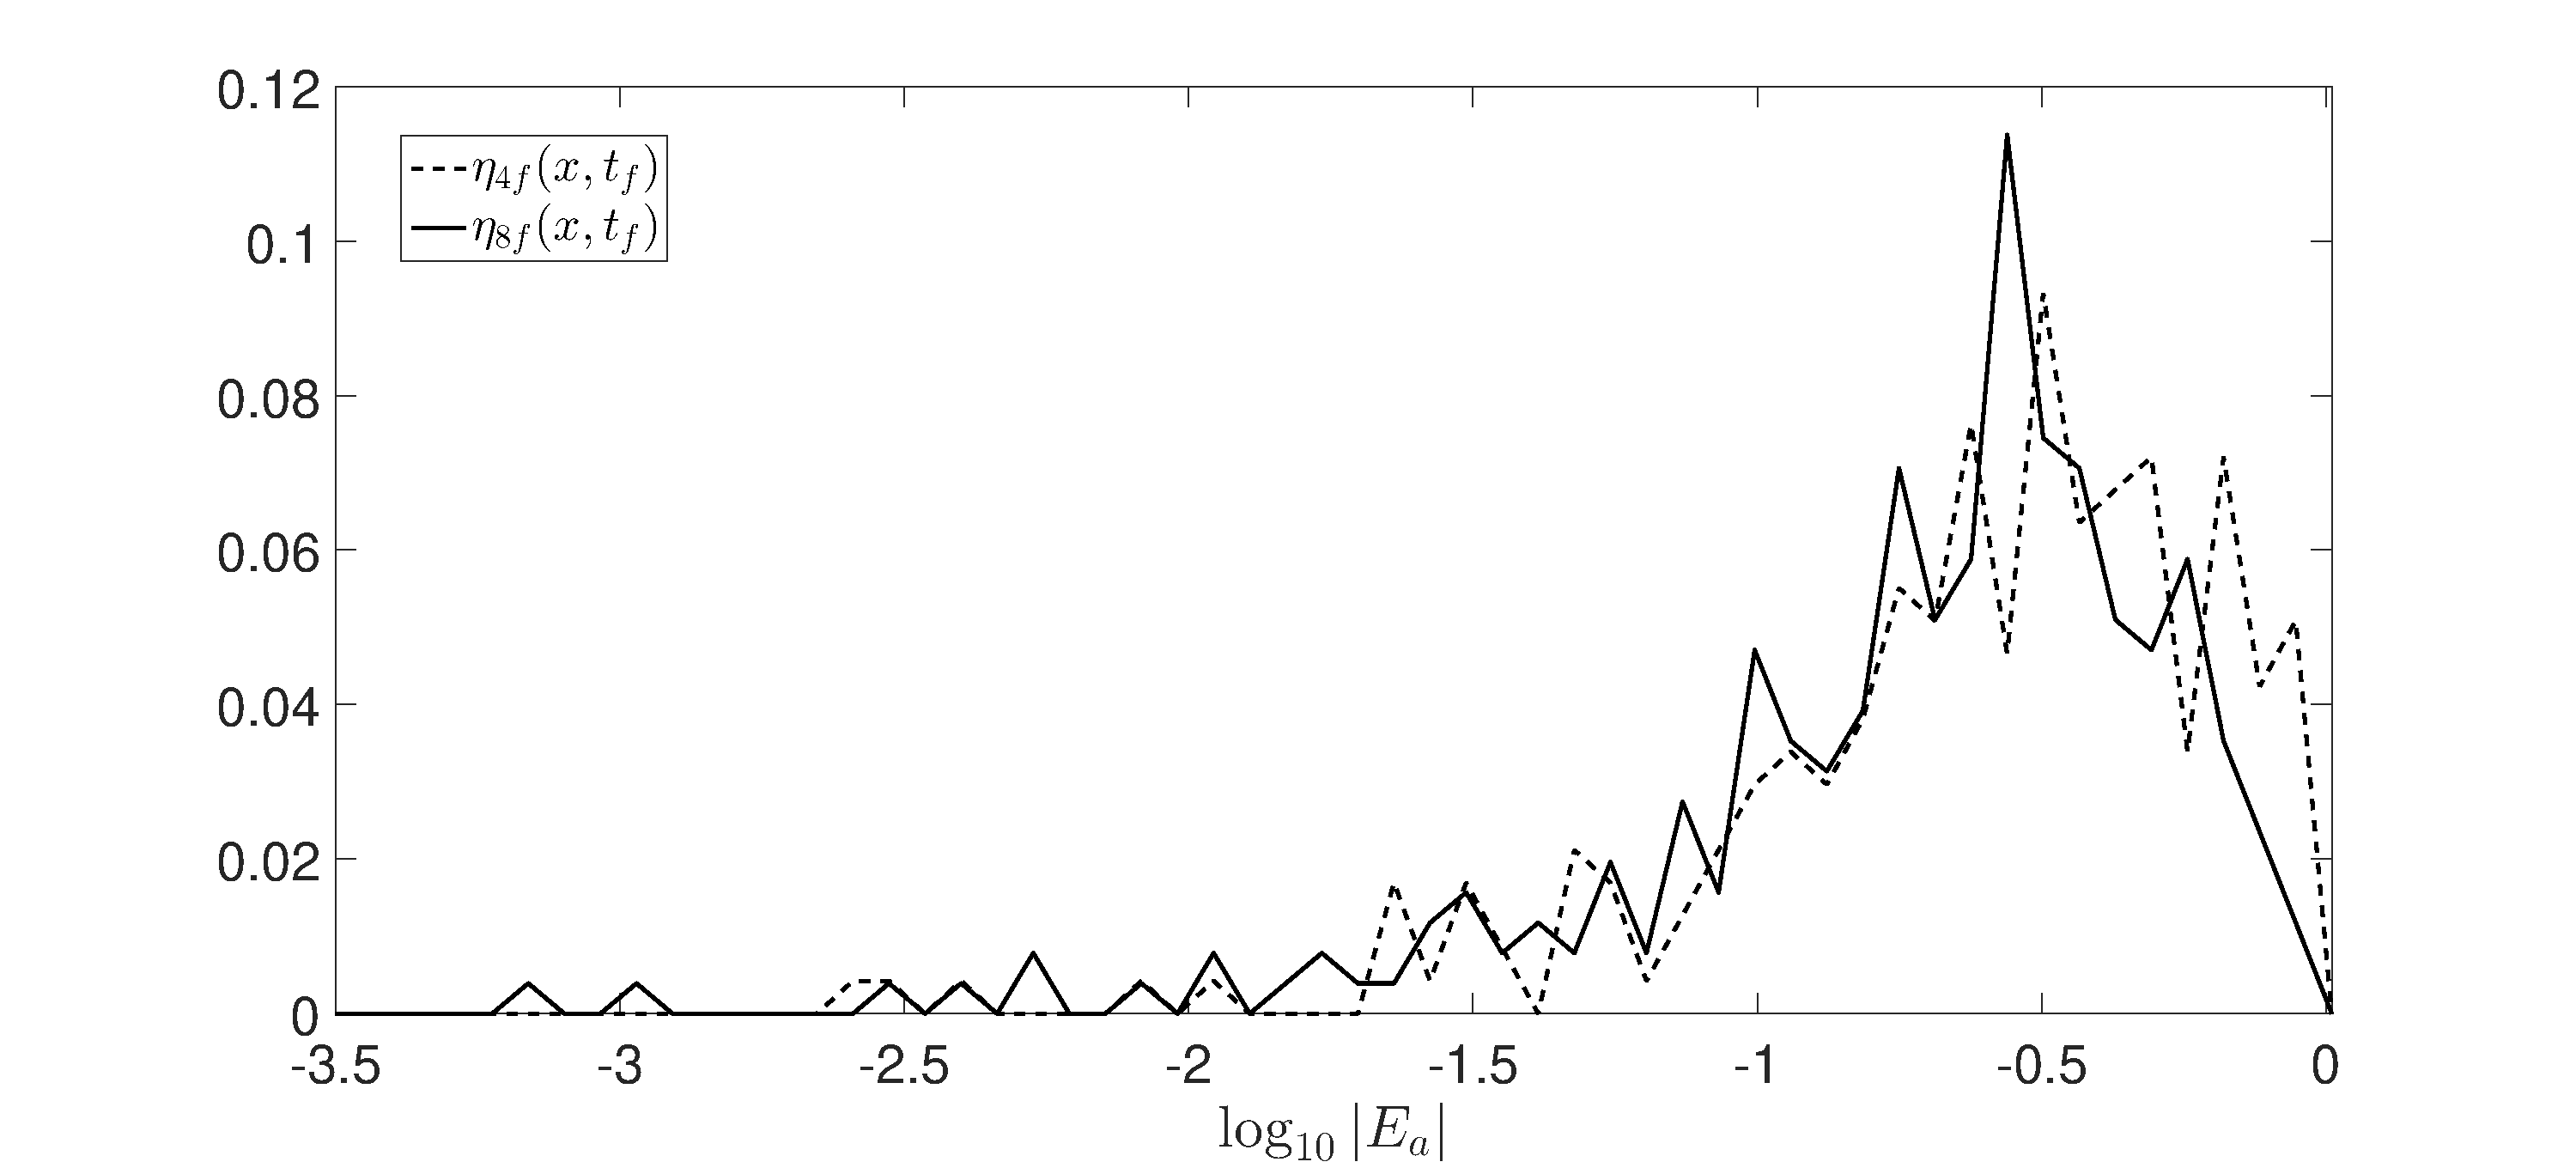
\includegraphics[width=.95\textwidth]{Images/histogram_tf_20_sig_pt1_4_vs_8floats_Mval_14}\\
		(b)\\
		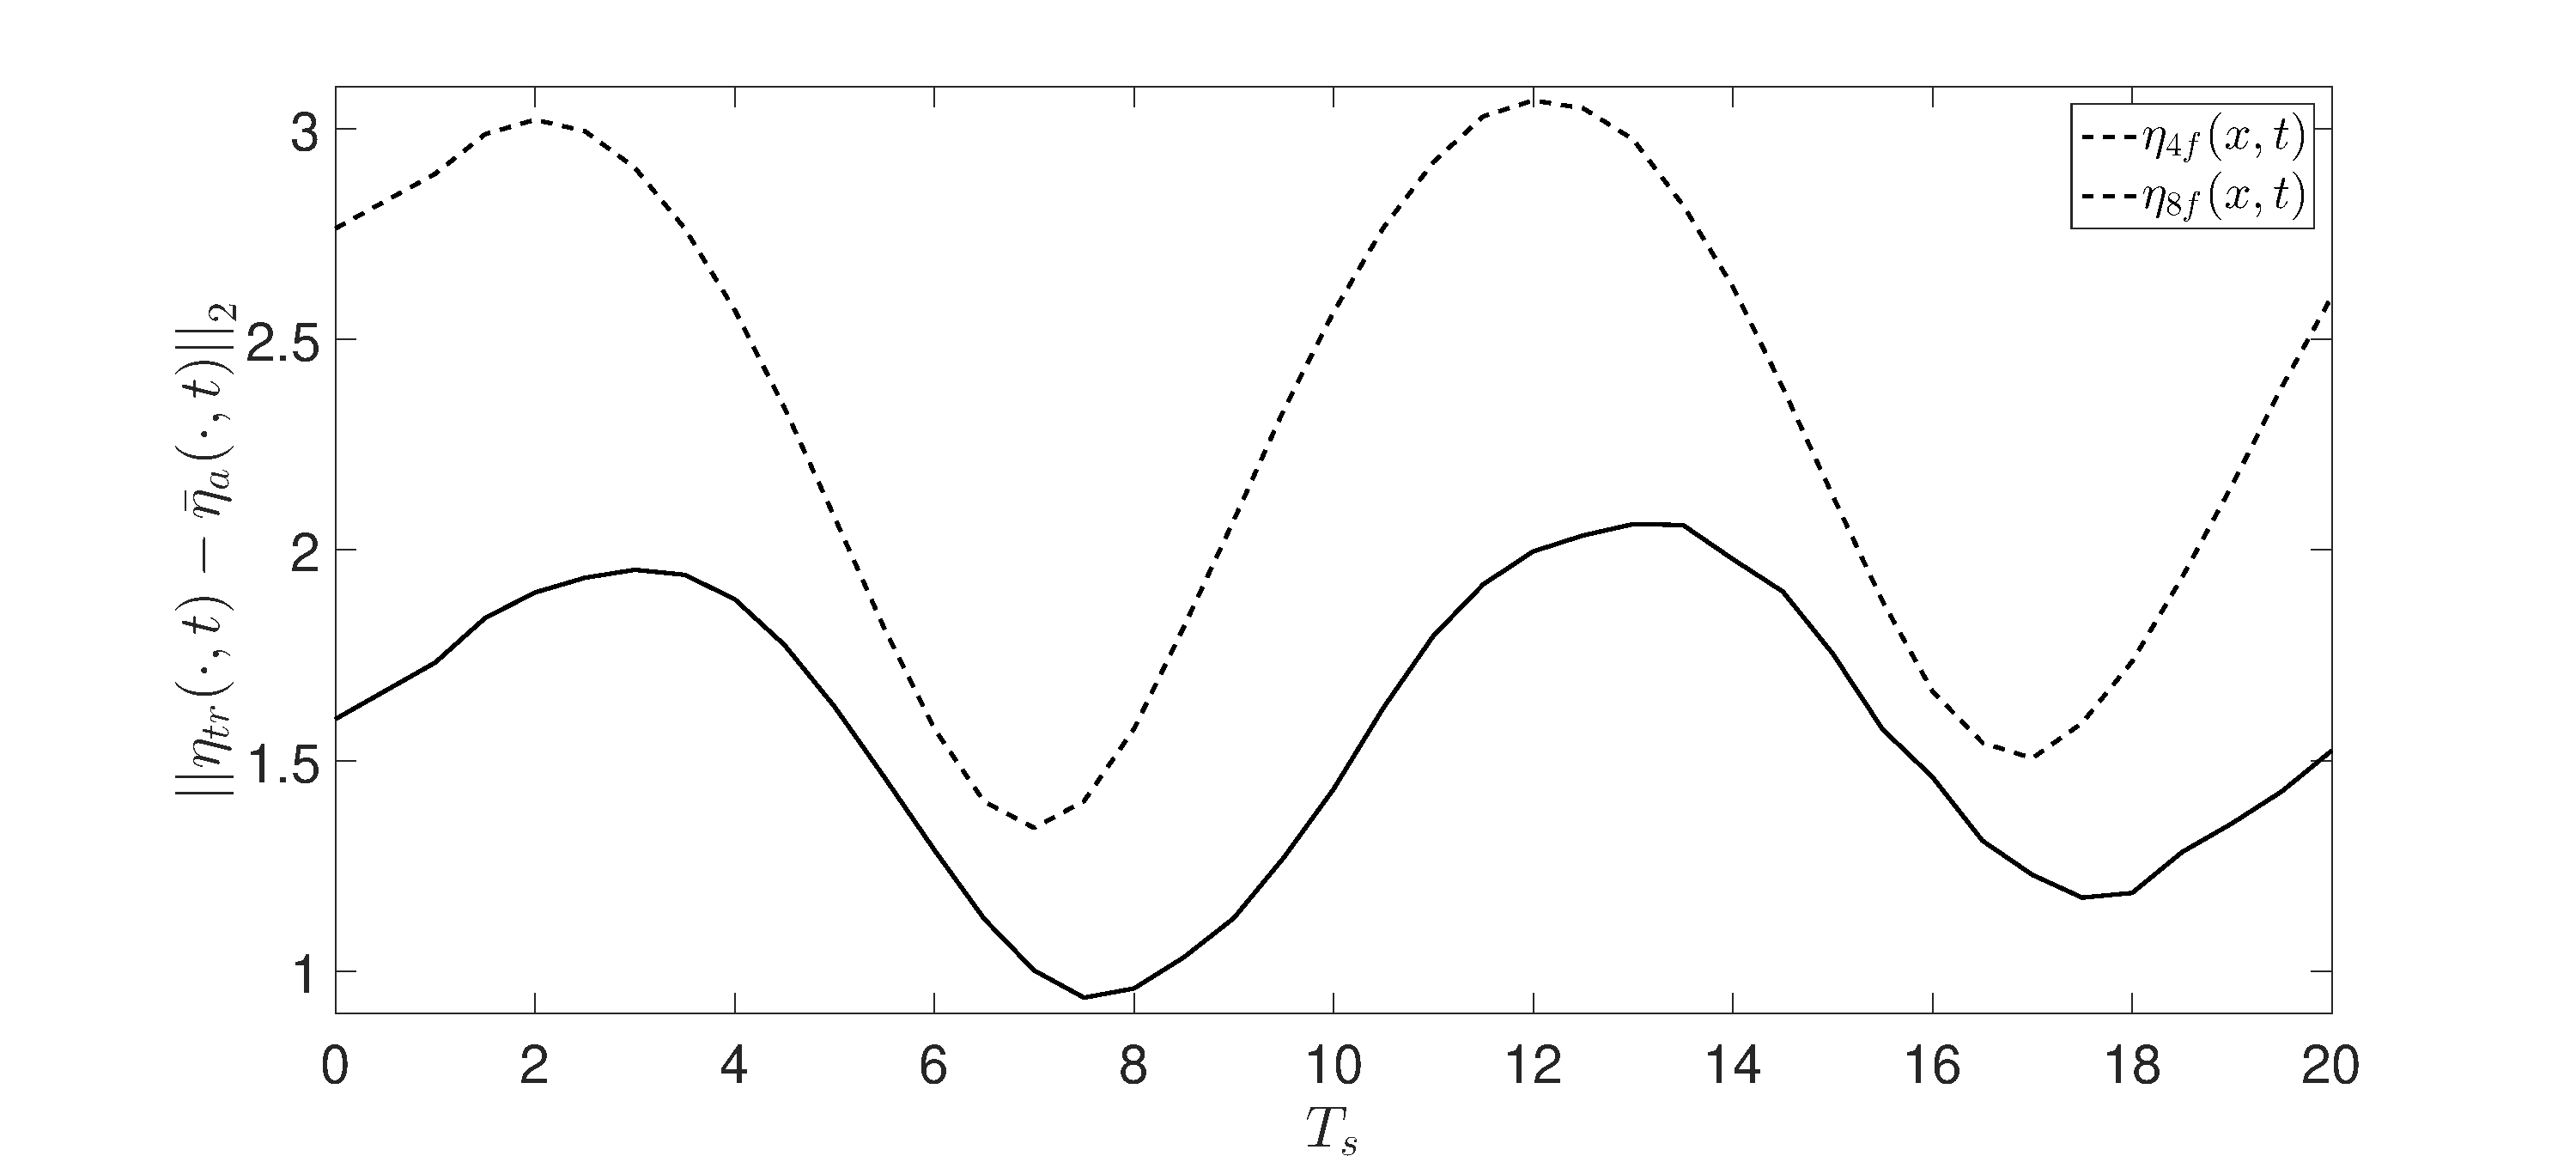
\includegraphics[width=.95\textwidth]{Images/rmserr_tf_20_sig_pt1_4_vs8floats_Mval_14}\\
		(c)
	\end{tabular}
	\caption{{\bf Lagrangian Assimilation} -For $M=14$, $dt_{s}=.5$, with four floats (--) compared to eight (-), we have the wave profiles at $t_{f}=20$ (a), a histogram of the log of the pointwise error (b), and the root-square error at every sampling time (c).} 
	\label{fig:Mval_14_lagran}
\end{figure}
